\documentclass[10pt,twocolumn,letterpaper]{article}

\usepackage{iccv}
\usepackage{times}
\usepackage{epsfig}
\usepackage{graphicx}
\usepackage{amsmath}
\usepackage{amssymb}

% Include other packages here, before hyperref.
\usepackage{graphicx}
\usepackage{pslatex}
\usepackage{subfigure}
\usepackage{amsmath}
\usepackage{amssymb}
\usepackage{tikz}
\usepackage{marvosym}
\usepackage{wasysym}
\usepackage{times}
\usepackage{epsfig}
\usepackage{tabularx}
\usepackage{enumitem}
\usepackage{sidecap}
\usepackage{verbatim}
\usepackage{makecell}

% If you comment hyperref and then uncomment it, you should delete
% egpaper.aux before re-running latex.  (Or just hit 'q' on the first latex
% run, let it finish, and you should be clear).
\usepackage[pagebackref=true,breaklinks=true,letterpaper=true,colorlinks,bookmarks=false]{hyperref}

% \iccvfinalcopy % *** Uncomment this line for the final submission

\def\iccvPaperID{****} % *** Enter the ICCV Paper ID here
\def\httilde{\mbox{\tt\raisebox{-.5ex}{\symbol{126}}}}

% Pages are numbered in submission mode, and unnumbered in camera-ready
\ificcvfinal\pagestyle{empty}\fi
\begin{document}

%%%%%%%%% TITLE

%%%%%%%%% TITLE
\title{Vision-based classification of developmental disorders using eye-movements}

\author{{\bf Guido Pusiol}
\texttt{pusiol@cs.stanford.edu}
Department of Computer Science\\
Department of Psychology \\
  \And {\bf Andre Esteva} 
\texttt{esteva@cs.stanford.edu} 
Department of Electrical Engineering
  \And {\bf Li Fei-Fei}
\texttt{feifeili@cs.stanford.edu} 
Department of Computer Science
   \And {\bf Michael C. Frank}
\texttt{mcfrank@stanford.edu}
Department of Psychology
   \And {\bf Scott Hall} 
\texttt{shall@stanford.edu}\\
  Department of Psychiatry\\
Stanford University}
  

\maketitle
% \thispagestyle{empty}

%%%%%%%%% ABSTRACT
\begin{abstract}
\noindent This paper proposes a system for classifying developmental disorders via measurements of individuals' eye-movements during naturalistic social interaction.
Using a new dataset of eye-tracking during interviews with patients, we build visual features that can distinguish between Fragile-X syndrome (a genetic disorder with Autism-like symptoms) and other idiopathic developmental disabilities. 
We design a one-dimensional convolutional neural network with state-vector inputs that outperforms a number of baseline systems, achieving 90\% precision on a subset of the data.
Fragile-X is an important case study for autism diagnosis because of the existence of gold-standard genetic diagnoses. By highlighting the existence of detectable visual patterns of social attention, our results suggest that these methods can be generalized to autism spectrum disorders more broadly and that they have the potential to assist medical practitioners in the diagnostic process. 
\end{abstract}
   
%%%%%%%%% BODY TEXT
\section{Introduction}
   
Autism Spectrum Disorder (ASD), is an important developmental disorder to account for and understand in our society today. Significant efforts are spent in early diagnosis, which is a key component to proper treatment.  Today, identification of a ASD requires a set of cognitive tests and hours spent on clinical evaluations which involve extensively testing the participant and observing their behavioral patterns (i.e. their social engagement with others). Physicians go through extensive training and require substantial experience to properly assess ASD.  The problem with this procedure is that it is both laborious and imprecise due to variability in the clinician's subjective judgement. With the advent of computers and machine learning techniques, people are beginning to look for computer-assisted technology to identify ASD. 

\begin{figure}[ht]   
\centering
\includegraphics[width=0.48\textwidth]{figures/Pull.png}
\caption{We perform gaze-tracking and facial-analysis to study participants (1) with mental impairments engaging in social interactions with an interviewer (2), that behave differently depending on their mental disorder. The goal of our work is to classify between disorders using this data.}
\label{fig:pull_figure}
\end{figure} 

In this work, we aim to create an automated system to assist physicians in the diagnosis of ASD (see Figure \ref{fig:pull_figure}). Specifically, we focus on Fragile-X-Syndrome (FXS). FXS is the most common known genetic cause of autism \cite{Hagerman:2008wg}, affecting approximately 1 in 3,000 individuals in the United States (approximately 100,000 people nationally). Individuals with FXS often show prominent eye gaze deficits during social encounters in which they actively seek to avoid social interaction \cite{Cohen:1988vx,Cohen:1989cm}. These social-attentional behavioral phenotypes are considered to be salient cues which drive investigations to better asses mental impairment \cite{Kennedy:2001dg}. 
   
Pioneering work by \cite{Rehg} shows the potential of using eye-tracking information to measure relevant behavior in children with ASD. However, it did not address the issue of distinguishing between ASD/FXS and other disorders in an automated way. Our work extends this to develop a vision-driven means for FXS classification via eye-tracking. Our data is video of an experimenter interviewing patients, overlaid with the patient's point of gaze (as measure by a remote eye-tracker). These participants have either FXS or some other developmental disorder (DD). We build descriptive features from this multi-sensorial data that capture social engagement between participant and experimenter. We then use these features to train classifiers to discern between different participants' disorder. One challenge is demonstrating that our features can help us better understand ASD. Another challenge is building an automated system capable of disambiguating between participants with different developmental conditions given the variability between individuals with the same disorder. 

Our contribution is a system capable of performing automatic assessment of the participant's developmental condition using a novel feature representation and a hand-crafted classifier that works well with our data. We perform quantitative analysis of our data in order to provide insight into the differences and variance in the behavioral patterns of these developmental conditions. Our results show that this system works with an accuracy well above chance, in some cases attaining 90\% precision. In addition, data analysis reveals that patterns in eye gaze considered at the fine granularity of facial regions (i.e. nose, mouth, etc.) are strong cues in describing a participant's diagnostic (Figure \ref{fig:pull_figure}). 

This paper is divided as follows. In section 2, we discuss prior work. In section 3, we describe the data: its collection and the sensors used. In section 4, we present an overview of the proposed system. In section 5, we describe the built features and analyze them. In section 6, we apply classification techniques and propose a new model. In section 7, we describe our approach for classifying the mental condition of an unknown participant. In section 8 we discuss the results and future work.

%%%%%%% PREVIOUS WORK %%%%%%%%
\section {Previous Work}

\subsection{Classification of disorders} Previous efforts in the classification of developmental disorders such as epilepsy and schizophrenia have relied on using electroencephalogram (EEG) and neurophysiological signals \cite{Kumar, sabeti}. These methods are accurate, but they suffer from long recording times and the use of EEG probes positioned all over a participants scalp and face. Meanwhile, eye-tracking has long been used to study autism and characterize the disease \cite{Boraston, hashemi, dalton}, but a rigorous automated system complete with visual feature extraction and classification has yet to be proposed. Here we propose a step towards an integrated approach to solving this problem. 

\subsection{Cognitive Impairment Studies} Individuals with FXS exhibit a set of developmental and cognitive deficits including impairments in executive functioning, visual memory and perception, social avoidance, communication impairments and repetitive behaviors \cite{Hall:2006jd,Pimentel:1999vx,Sullivan:2007gz,Sullivan:2006jc}. In particular \cite{Hall:2012ge} shows that eye-gaze avoidance during social interactions with others is a salient behavioral feature of individuals with FXS. Maintaining appropriate social gaze is critical for language development, emotion recognition, social engagement, and general learning through shared attention \cite{Csibra:2006wf, Morales:2000br,Emery:2000ug}. Studies have indicated that high levels of gaze avoidance are characteristic of poor social interaction skills \cite{DohertySneddon:2013fv,Riby:2012il}. For instance, when shown images of faces depicting various emotions, participants with FXS looked significantly less at the eye region of the faces, and were more likely to look at the nose region compared to healthy individuals. Despite this, few researchers have attempted to employ eye-tracking methodology to quantify social gaze behavior in real-life social settings \cite{Farzin:2009fq, Farzin:2011ip}.   Limitations of previous studies include a small sample of participants and the fact that the controls were not matched on level of cognitive functioning to the participants with FXS. As such, in the present study we utilize data in which a larger group of individuals with FXS (both males and females) were studied and in which controls were cognitively matched.

\subsection{The mechanism for human visual attention} It is commonly believed that visual attention is driven by two mechanisms: 1) A bottom-up (BU), task independent, image-based mechanism that instinctively guides the human eyes into salient image regions such as discontinuities, color, texture, motion, etc. \cite{AmodelofsaliencybasedvisualattentionforrapidsceneanalysisItti:tq}, 2) A top-down (TD)  mechanism that guides attention and gaze in a task-dependent and goal-directed fashion, that is able to manage the sequential acquisition of information from the visual environment \cite{HANDEYE, Borji:2012dq}. We focus on this second category and investigate the underlying visual structures behind social interaction engagement. Despite its importance in understanding human behaviors, only a few approaches have addressed this TD mechanism. Previous TD work tackles the problem of predicting gaze position using a head mounted monocular camera \cite{Fathi:2012vk}. There the goal was to mimic eye-tracking information with egocentric video information and not to understand human behavior. Egocentric activity detection by predicting hand-object interactions from a head-mounted camera \cite{Fathi:2013tc} has been addressed, as has social event detecting by facial direction analysis \cite{FromEgotoNosVisionDetectingSocialRelationshipsinFirstPersonViewsAlletto:wi}. Previous work has addressed the problem of understanding cognitive and motivational factors of the person wearing the eye tracker using manual analysis of the data \cite{linda}. To the best of our knowledge, automated classification of cognitive impairments using eye-tracking data remains an unaddressed problem.  In this work we build unique features that capture moments of joint attention for the automatic screening and diagnosis of mental conditions.  
 
 %%%%%%%%% DATASET %%%%%%%%%%
\section{Dataset}

\subsection{Participants}
Participants were patients diagnosed with either an idiopathic developmental disorder or Fragile-X-Syndrome (FXS). There are known gender-related behavioral differences between FXS participants, so we further subdivided this group by gender into males (FXS-M) and females (FXS-F). There were no gender-related behavioral differences in the DD group, and genetic testing confirmed that DD patients did not have FXS. Patients were between 12 and 28 years old, with 51 FXS patients (32 male, 19 female) and 19 DD patients. The two groups were well-matched on chronological and developmental age, and had similar mean scores on the Vineland Adaptive Behavior Scales (VABS), a well-established measure of developmental functioning. The score was 58.47 (std = 23.47) for individuals with FXS and 57.68 (std = 16.78) for controls, indicating that the level of cognitive functioning in the two groups is almost 3 standard deviations (std) below the mean.

%a well-established measure of developmental functioning. The VABS adaptive behavior composite standard score was 58.47 (SD = 23.47) for individuals with FXS and 57.68 (SD = 16.78) for controls, indicating that the level of cognitive functioning in the two groups was almost 3 standard deviations below the mean.

\subsection {Environmental Set-Up}
The participants were each interviewed for a period of $\sim$10 minutes by a health professional interviewer. The interviews were conducted in a room with minimal visual distractions to control for the participants' attention. The distance between the participants and the interviewer was $\sim$1.5m. Figure \ref{fig:environment} depicts the the environment configuration. The eye-tracker and the camera are synchronized in time. A linear transformation maps the coordinate values of the eye-tracker to the coordinate space of the camera.  

\begin{figure}[ht]   
 \centering
           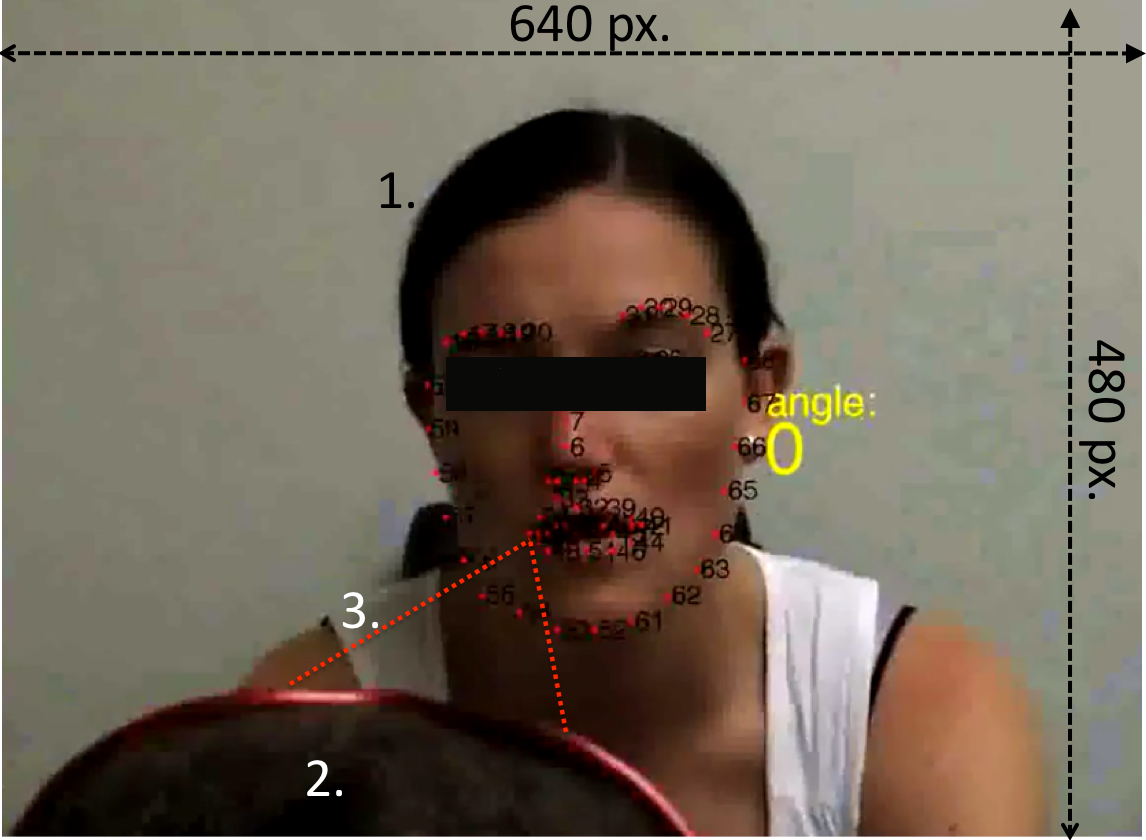
\includegraphics[width=3.2in,height= 2.4in]{figures/Real.png}
 \caption{A frame from videos showing the participant's view (participant's head is visible in the bottom of the frame). Eye-movements are tracked with a remote eye-tracker and mapped into the coordinate space of this video.}
\label{fig:environment}
\end{figure}

%%% SECTION: SYSTEM ARCHITECTURE %%%%
\section{System Architecture}
The assistive system takes as input multi-sensorial eye-tracking and video data and outputs a prediction on the mental disorder of the participant. Figure \ref{fig:system_architecture} depicts the architecture of the system. It is composed of the following three parts, elaborated further in sections \ref{sec:feature_extraction}, \ref{sec:classification}, \ref{sec:participant_classification}:

\textbf{Feature Extraction}. We build our features by mapping the eye-tracking information onto facial regions of the interviewer. 

\textbf{Training of Classifier}. We define and build classification models based on these features to label sequences of features as belonging to a particular mental condition.  

\textbf{Participant Classification}. We define a method to predict the condition of a new participant using these models. 

\begin{figure}
          \subfigure[]{
             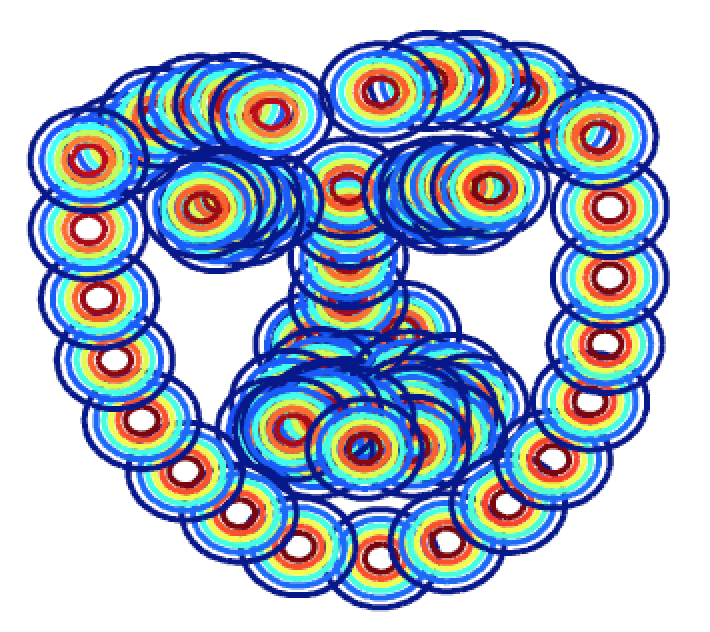
\includegraphics[width=0.6in,height=0.7in]{figures/movement1.png}
             } 
                  \hfill   
            \subfigure[]{
            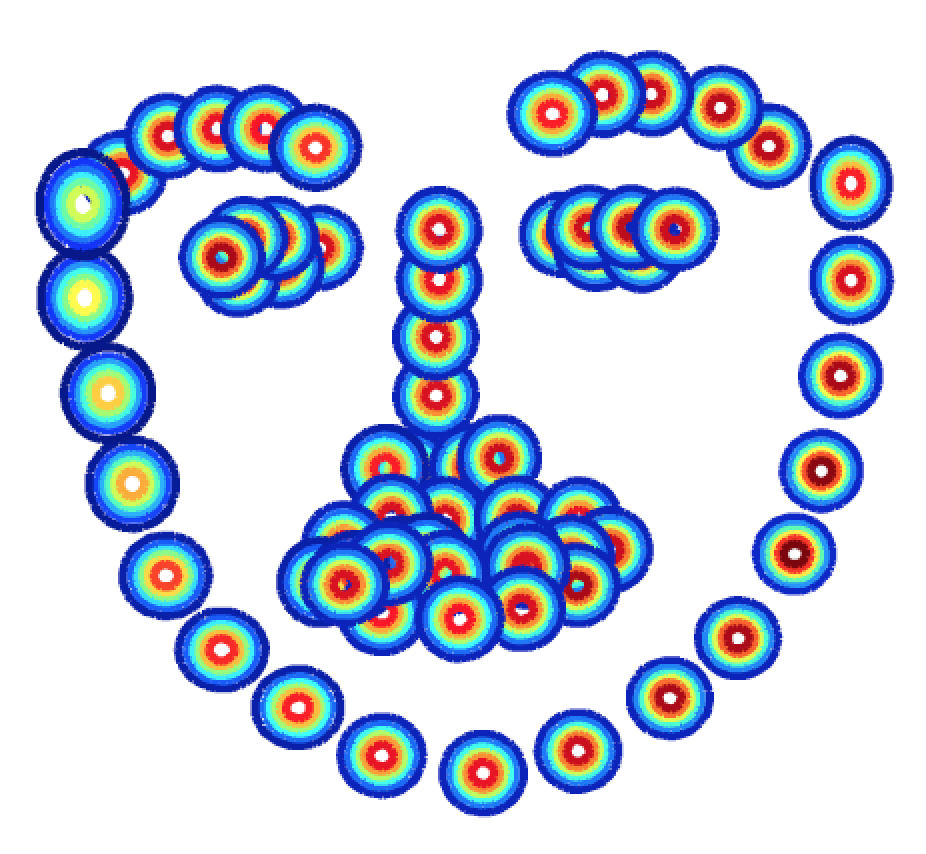
\includegraphics[width=0.6in,height= 0.7in]{figures/movement2.png} 
            }
                 \hfill
             \subfigure[]{
            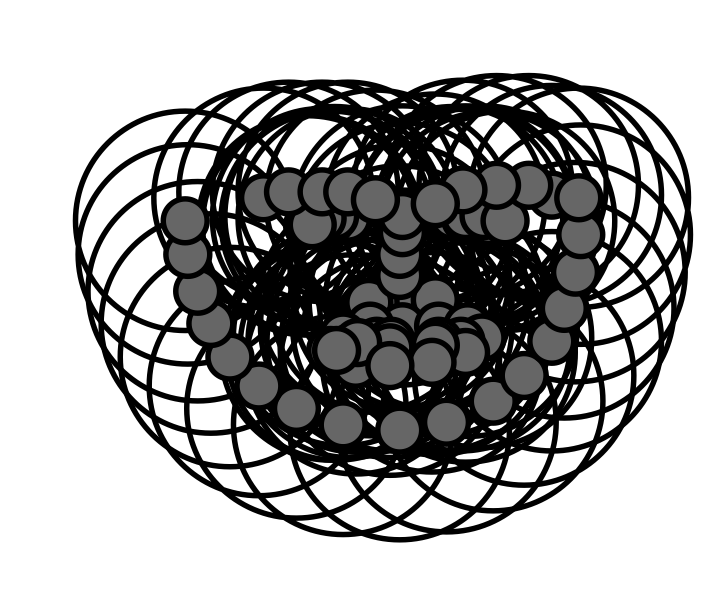
\includegraphics[width=0.6in,height= 0.7in]{figures/margin.png} 
            }
                 \hfill
             \subfigure[]{
            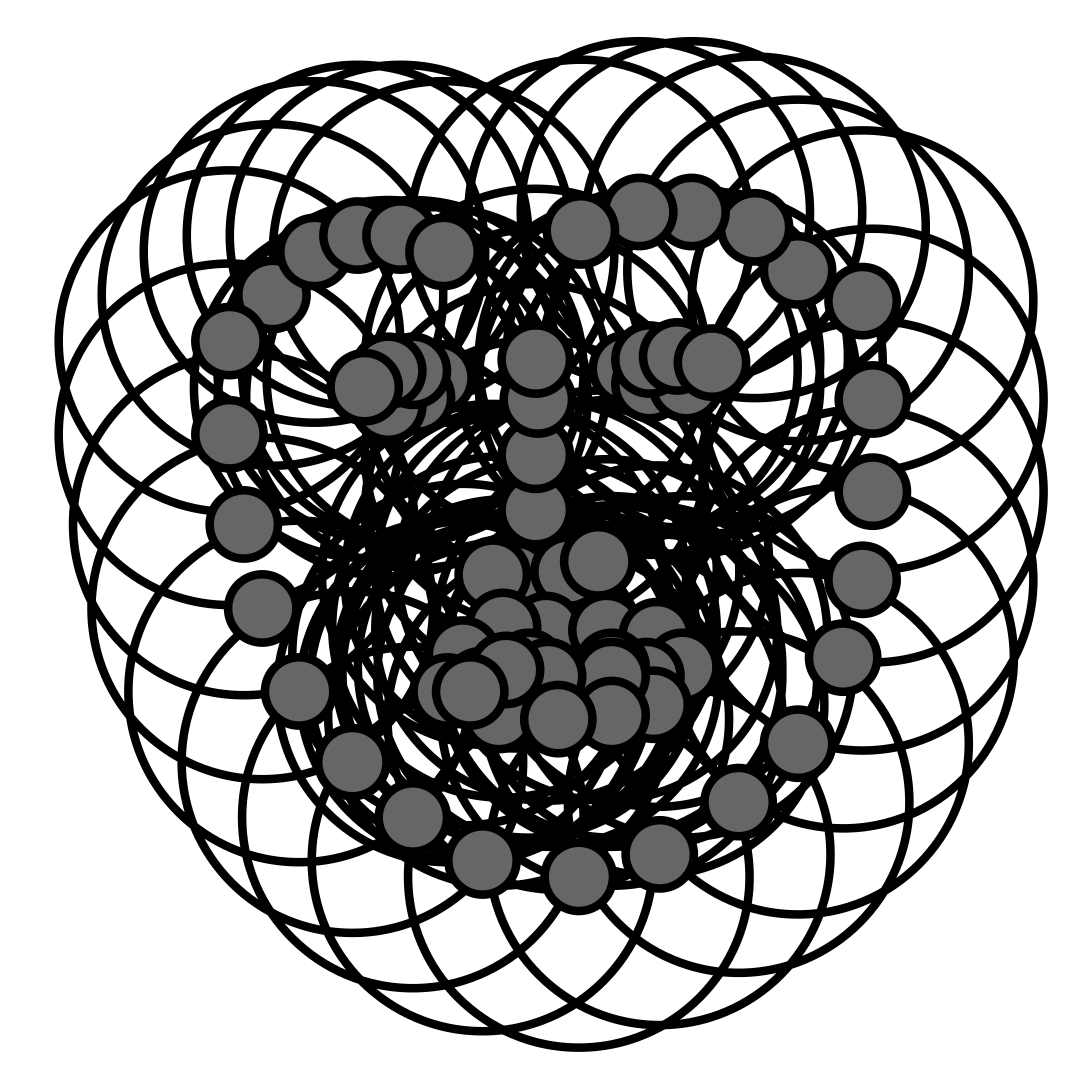
\includegraphics[width=0.6in,height= 0.7in]{figures/margin2.png} 
            }
    \caption{Face Motion Analysis. (a) The worst case of high motion of the interviewer; (b) the most steady interviewer. In all cases the interviewers are instructed to limit their head movement as much as possible; (c) and (d) represent the 20 px threshold radius surrounding the face key points. This threshold results in full face coverage across all interviews.}
\label{fig:PERSON}
\end{figure}

\begin{figure*}[ht]   
\centering
           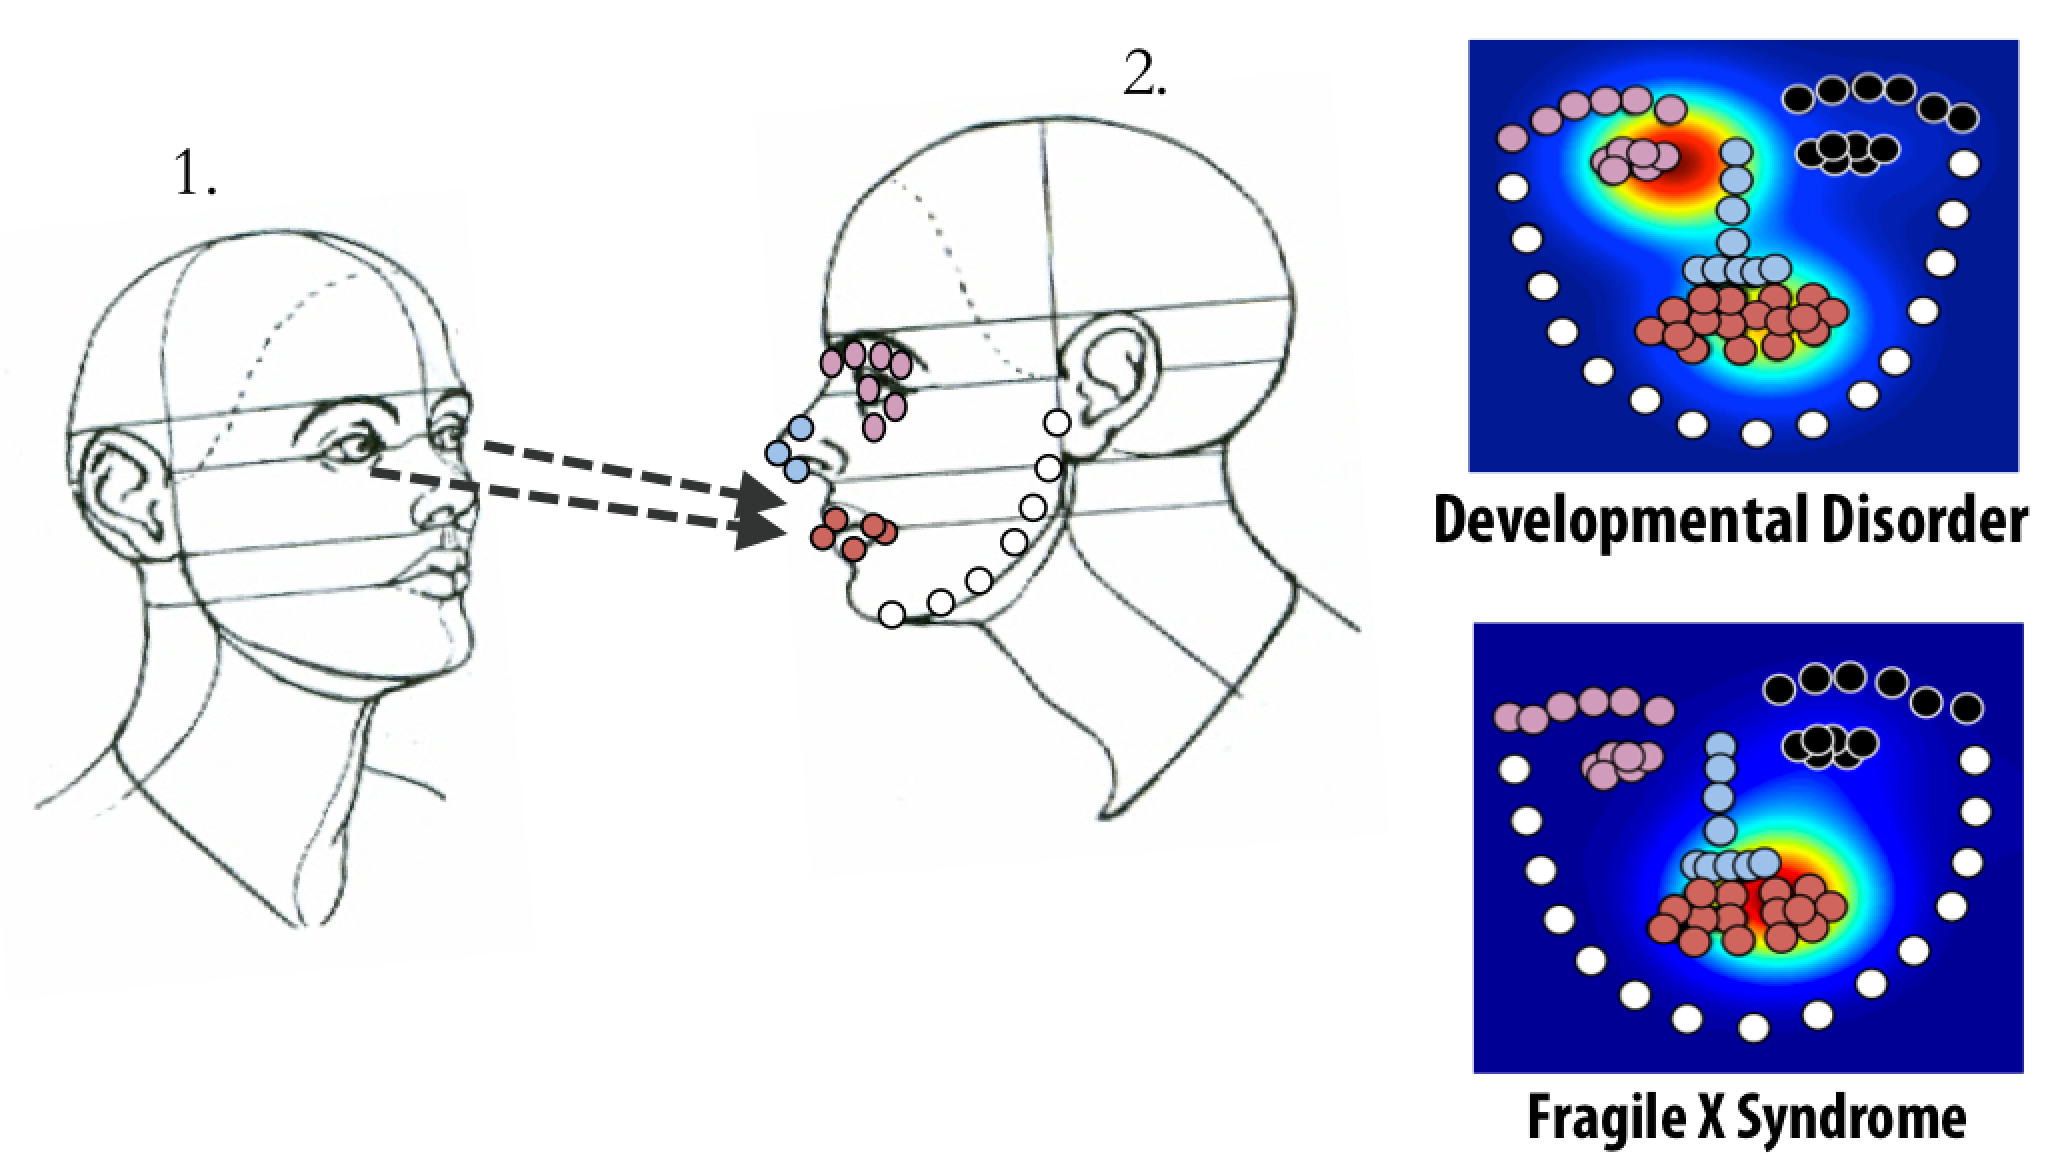
\includegraphics[width=\textwidth]{figures/system.png}           
 \caption{System Architecture. The environment is composed of an interviewer (1) facing a participant (2) who wears a remote eye-tracker (3) while a fixed-camera (4) faces the interviewer. Face marks (5) on the interviewer's face are extracted from the raw video and we map the eye-tracking data onto these marks. This mapping is then clustered into semantic facial regions (6) and we represent these facial regions using state vectors (7). Sub-sequences of features (8) are used to train classification algorithms (9). Finally, the full feature sequences of  unseen participants (10) are used to predict their mental disorder (11).}
\label{fig:system_architecture}
\end{figure*}

%%%% SECTION: FEATURE EXTRACTION %%%%%
\section{Feature Extraction}
\label{sec:feature_extraction}
A goal of our work is to build proper descriptive features that simultaneously provide insight into these disorders and allow for accurate classification between them. These features are the building blocks of our system, and the key challenge is engineering them to properly distill the most meaningful parts out of the raw eye-tracker and video footage.  

\subsection{Face-mark Extraction}
For each video frame we compute a set of face marks on the face of the interviewer using a deformable-parts-model based approach \cite{dpmface}. We reduce the bias of the interviewer by filtering out the frames where the interviewer is not facing the participant. This represents $<$1\% of all frames.

We have computed 58,587 frames for the 19 developmental disorder participants, 56,109 frames for the 19 FXS-female participants, 94,214 frames for the 51 FXS-Male participants. Our frame-rate is 5 frames per second. At each frame we compute 69 face-marks which total  14,414,790 marks over all frames. This was achieved using 500 cores over 96 hours. Face-mark quality was evaluated on a sample of 1000 randomly selected frames, out of which only a single frame was incorrectly annotated. Figure \ref{fig:environment} shows an example of face-marks extracted and displayed on the face of an experimenter during an interview. Figure \ref{fig:PERSON}(a)(b) shows examples of the spacial translation of the face-mark on two interviews. We can see that the interviewer's face is spatially stable during the interview and that these results are consistent across the interviews. 
 
\subsection{Feature Construction}
\label{ssec:feature_construction}
The eye-tracking system is calibrated to the camera coordinate system. We map the eye-tracking coordinates and the face marks with a linear transformation. The binding between the eye-tracking and the face-mark happens when the eye-tracking is within a 20 px. radius to the closest face-mark - Figure \ref{fig:PERSON}(c)(d). This value is manually defined to cover the interviewer's entire face.



\begin{figure}[h]
    \begin{center}
        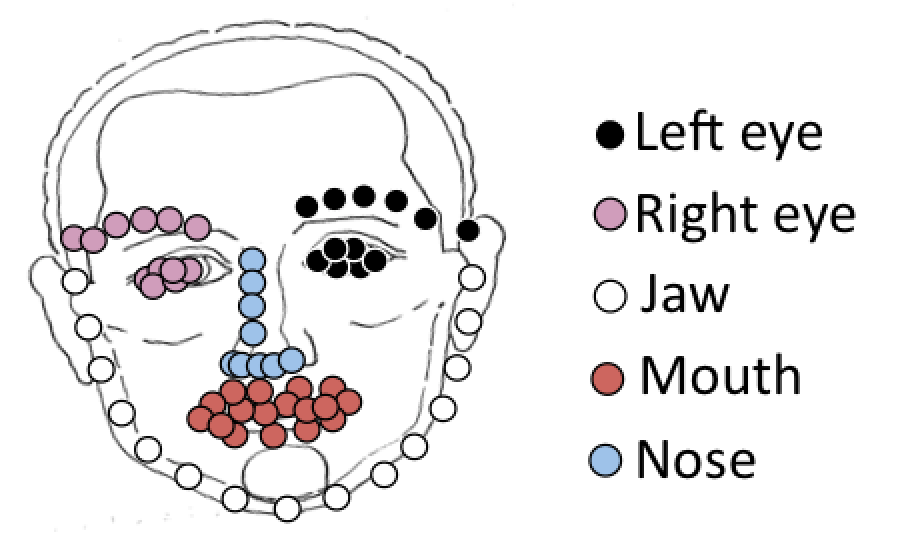
\includegraphics[width=0.5\linewidth]{figures/face2.png}
    \end{center}
    \caption{Clustering of the 69 key-marks of the interviewer's face into 5 semantic facial regions. The colors represent the clustering of these marks into 5 facial regions. A 6th region, not shown, is reserved for when the participants look away from the face. These clusters represents our features.}
    \label{fig:feats}
\end{figure}
We cluster the 69 facemarks into 6 regions: \textit{not looking at the face, nose, left-eye, right-eye, mouth, jaw}. Figure \ref{fig:feats} depicts this. 
We represent these regions as state vectors, as shown in Figure  \ref{fig:statevectors}, to emphasize the independence of facial regions.

%To convert this time-series into temporal features for learning algorithms we select a time-window of length \textit{n} and a time-step \textit{s} to form a feature matrix as follows: 
%\begin{enumerate}
%\item Form a temporal feature by selecting \textit{n} time-consecutive semantic tokens
%\item Slide the window across the time-series by a length \textit{s}
%\end{enumerate}

\begin{figure}[b]
        \centering
             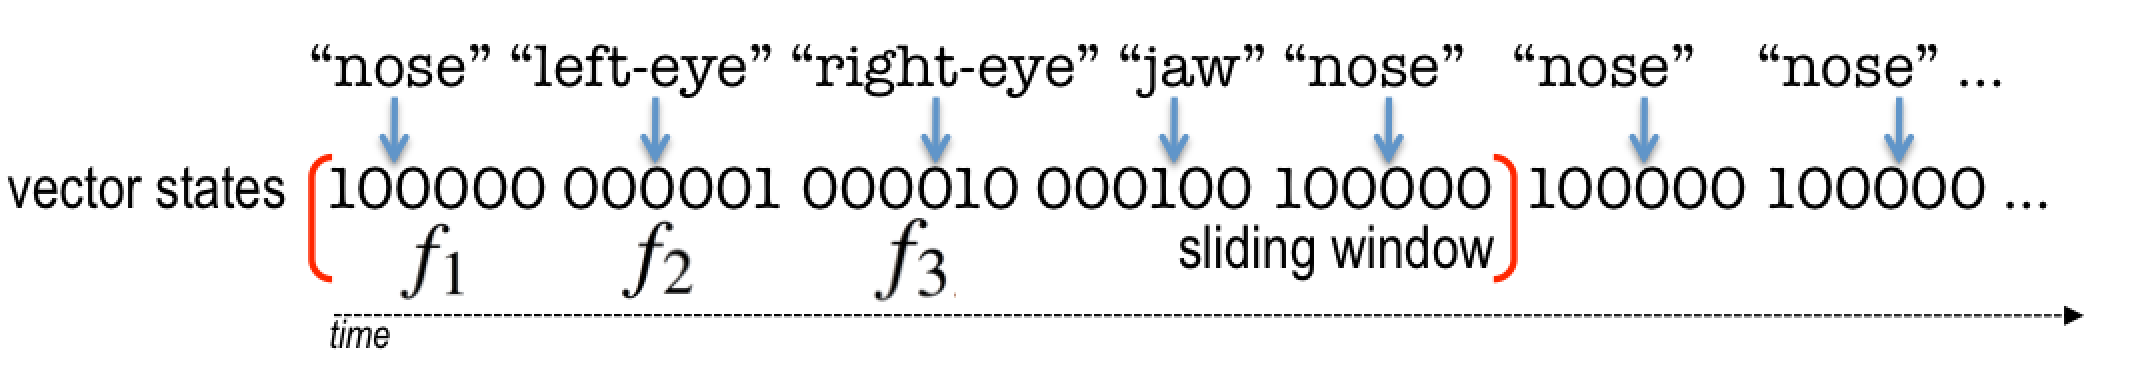
\includegraphics[width=0.5\textwidth]{figures/vectors.png}
       \caption{Facial Region State Vectors. The 5 facial regions and the non-face region are represented as state-vector features $f_i$. A sliding window technique is used to extract the input into our classifiers.}
        \label{fig:statevectors}
\end{figure}

\subsection{Notation} 
\label{sec:notation}
We define a feature $f$ to be a 6-element state vector (i.e. $f=<1,0,0,0,0,0>$) representing the 6 facial regions and $\bar{f} \in \{0,1,2,3,4,5\}$ to be its corresponding integer-valued representation. For participant $p^\alpha$, represented by the sequence of features $f_i$ as
\begin{equation}
p^\alpha=[f_1^\alpha, f_2^\alpha,....f_{T_\alpha}^\alpha]
\end{equation}
where $\alpha$ indexes the participants and $T_\alpha$ represents the length of the time series, we consider the set of all individuals of a given class $c$ to be
\begin{equation}
S_c=\{p^1, p^2,...p^N \}
%=\{f_1^1, f_2^1,....f_{T_1}^1, f_1^2, f_2^2,....f_{T_2}^2,... f_1^N, f_2^N,....f_{T_N}^N\}
\end{equation}
 where $c$ indexes \{DD, FXS-female, FXS-male\}.
\subsection{Descriptive Analysis}

We next briefly present a number of descriptive analyses of the dataset that explore the complexity of this rich data and justify the importance of using temporal information in classification.

\subsubsection{Fourier Analysis of Features}
We consider the spectra of the time-series for each group (DD, FXS-male, FXS-female) by concatenating the integer-representation time-series of each patient $\bar{p}^\alpha=[\bar{f}_1^\alpha, \bar{f}_2^\alpha,....\bar{f}_{T_\alpha}^\alpha]$ of the group into one time-series $\bar{S}_c=\{\bar{p}^1, \bar{p}^2,...\bar{p}^N \}$ and taking the Fourier transform. What we find is that each group exhibits strong near-zero-frequency components with weak and noisy higher order components. We further find that the spectra of the signal after eliminating the non-face state vectors has the same pattern. This implies that there exist no characteristic oscillatory movements in the data and that participants tend either to fixate to a single region of the face or scan across multiple regions. 

\subsubsection{Feature Granularity}

It is clinically relevant to analyze the distribution over time of the attention of the participants to different regions of the face.  As seen in Figure \ref{fig:histo}, participants spend the majority of the interview looking away from the interviewer, and only a fraction of the time looking at the interviewer's face. Considering the feature distribution over the face, Figure \ref{fig:histo}(d)-(f), we see that DD and FXS-F are quite similar, whereas FXS-M is distinct. FXS-M focuses primarily on mouth (4) and nose (1) areas. This justifies the use of a finer granularity of face regions to construct features as opposed to coarser features based on whether or not individuals are looking at the face.
\begin{figure}%[t]
          \subfigure[ DD]{
             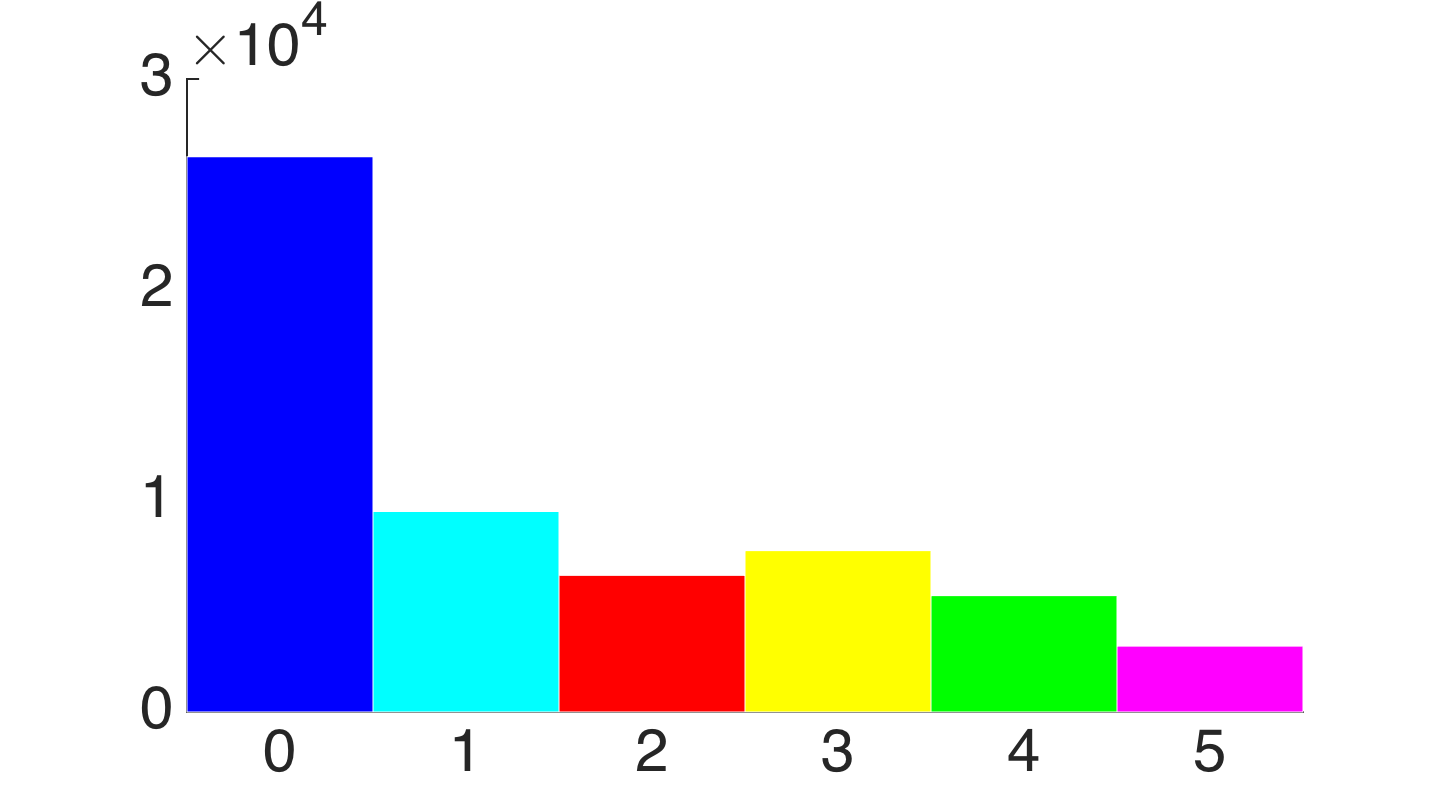
\includegraphics[width=1in,height= 0.7in]{figures/semdd.png}
             } 
               \hfill   
            \subfigure[FXS-F]{
            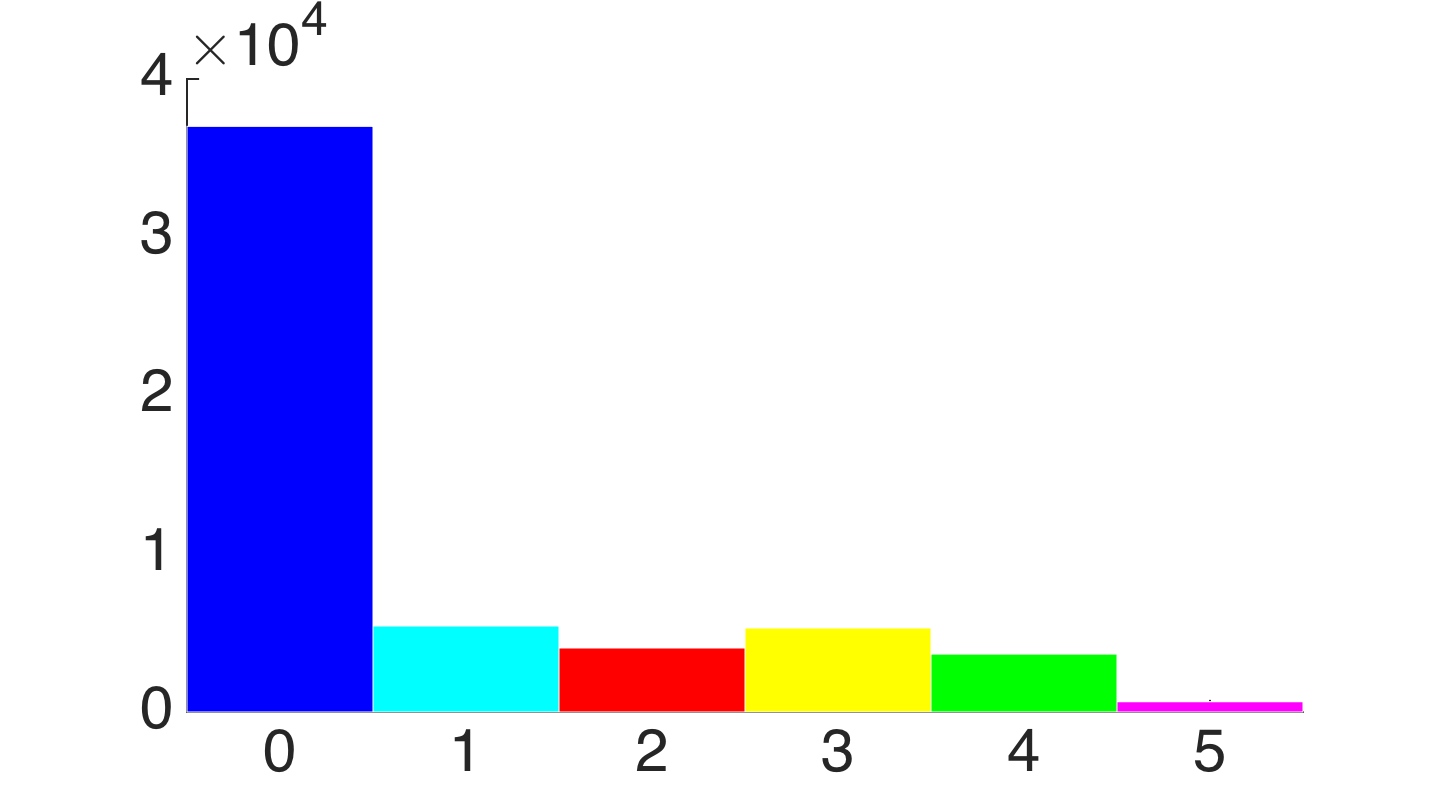
\includegraphics[width=1in,height= 0.7in]{figures/semfemale.png} 
            }
               \hfill
             \subfigure[FXS-M]{
            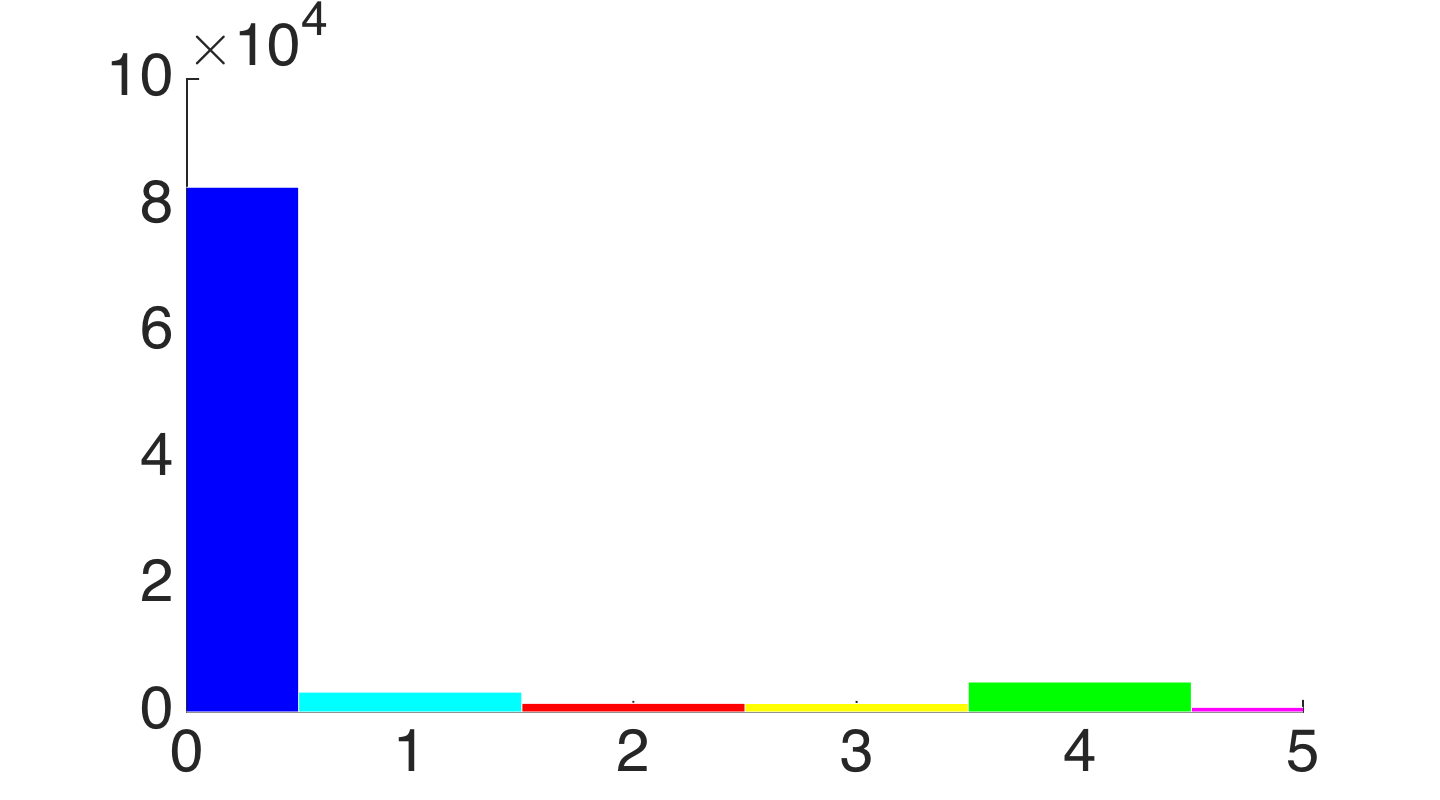
\includegraphics[width=1in,height= 0.7in]{figures/semmale.png} 
            }
          \subfigure[DD]{
             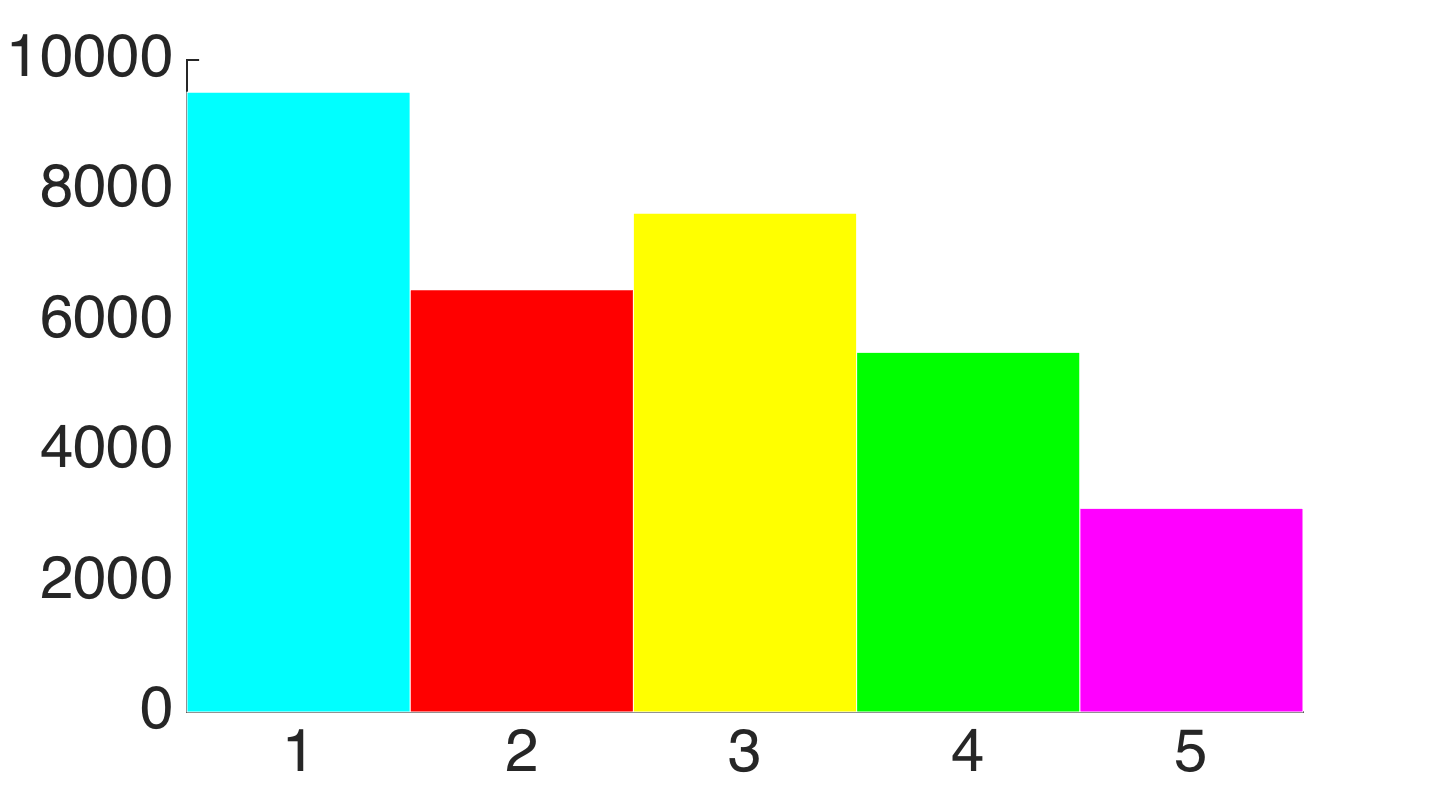
\includegraphics[width=1in,height= 0.7in]{figures/semdd-face.png}
             } 
               \hfill   
            \subfigure[FXS-F]{
            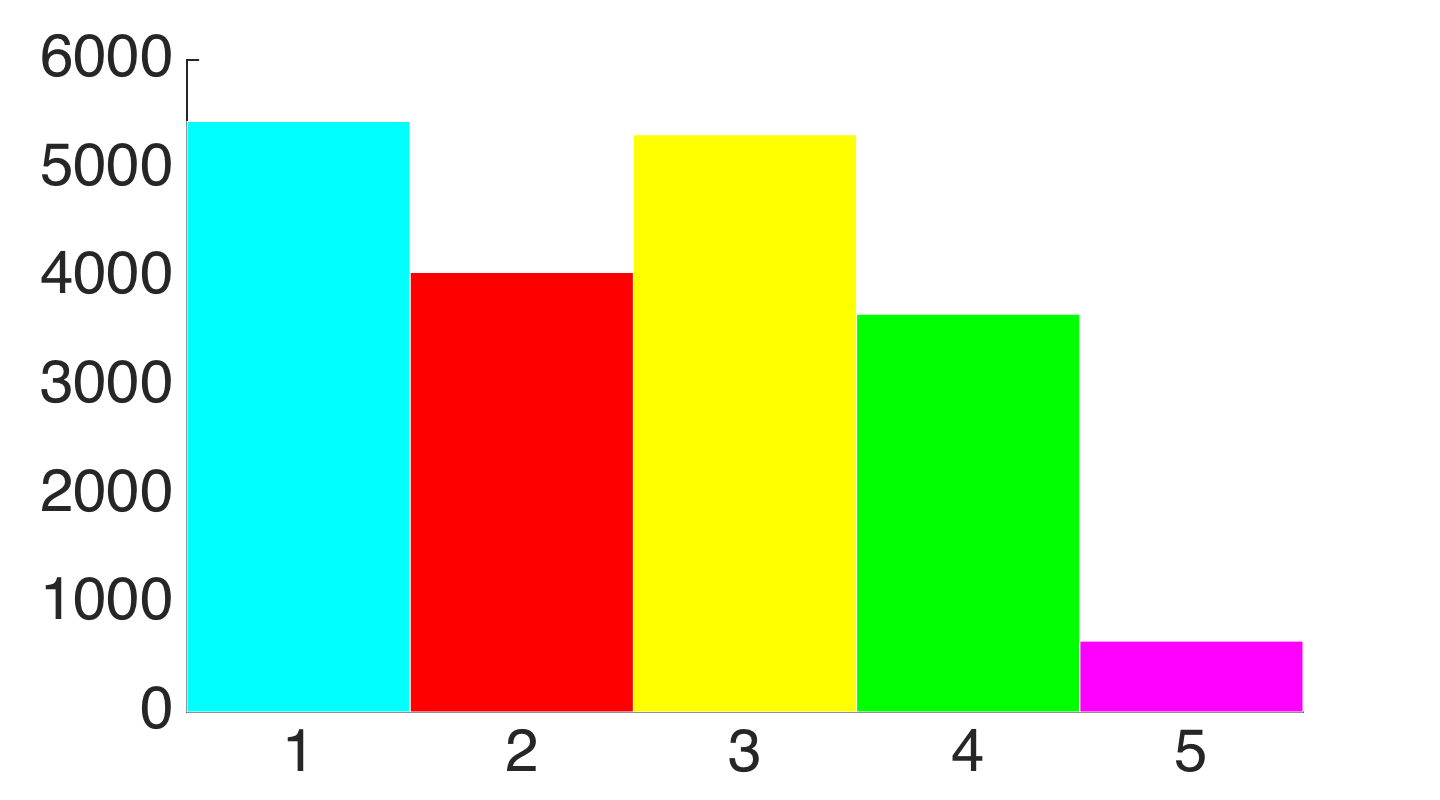
\includegraphics[width=1in,height= 0.7in]{figures/semfemale-face.png} 
            }
               \hfill
             \subfigure[FXS-M]{
            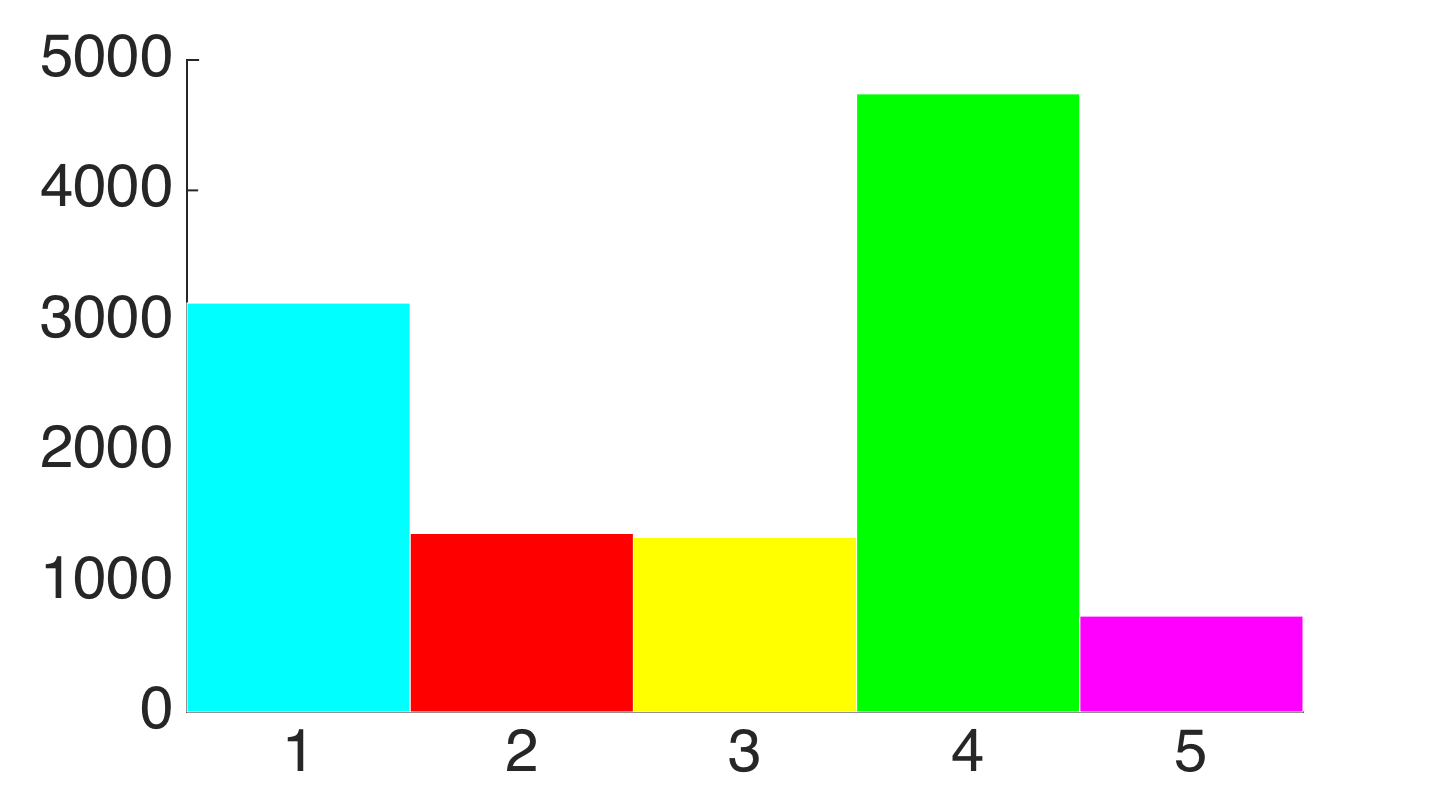
\includegraphics[width=1in,height= 0.7in]{figures/semmale-face.png} 
            }
            
\caption{Feature histograms for the various disorders. X-axis represents different states: non-face (0), nose (1), eye-left (2), eye-right (3), mouth (4), and jaw (5). (a)-(c) feature histograms for all participants of each class. (d)-(f) equivalent histograms with the non-face state vector removed.}
\label{fig:histo}
\end{figure}


\subsubsection{Attentional transitions}
It is also clinically relevant to analyze the transitions between facial regions in time. Figure \ref{fig:transitions} shows these transitions in a color map. We find a marked difference between the different disorders. Individuals with DD exhibit greater counts of transitions, whereas those with FXS exhibit significantly less. The transitions between facial regions better identify the three groups than the transitions from non-face to face regions. FXS-M participants tend to swap their gaze quite frequently between mouth and nose, whereas the other two do not. DD participants exhibit much movement between facial regions, without any clear preference. FXS-F patterns resemble DD, though they are much less pronounced.

\begin{figure}[b]
          \subfigure[DD]{
             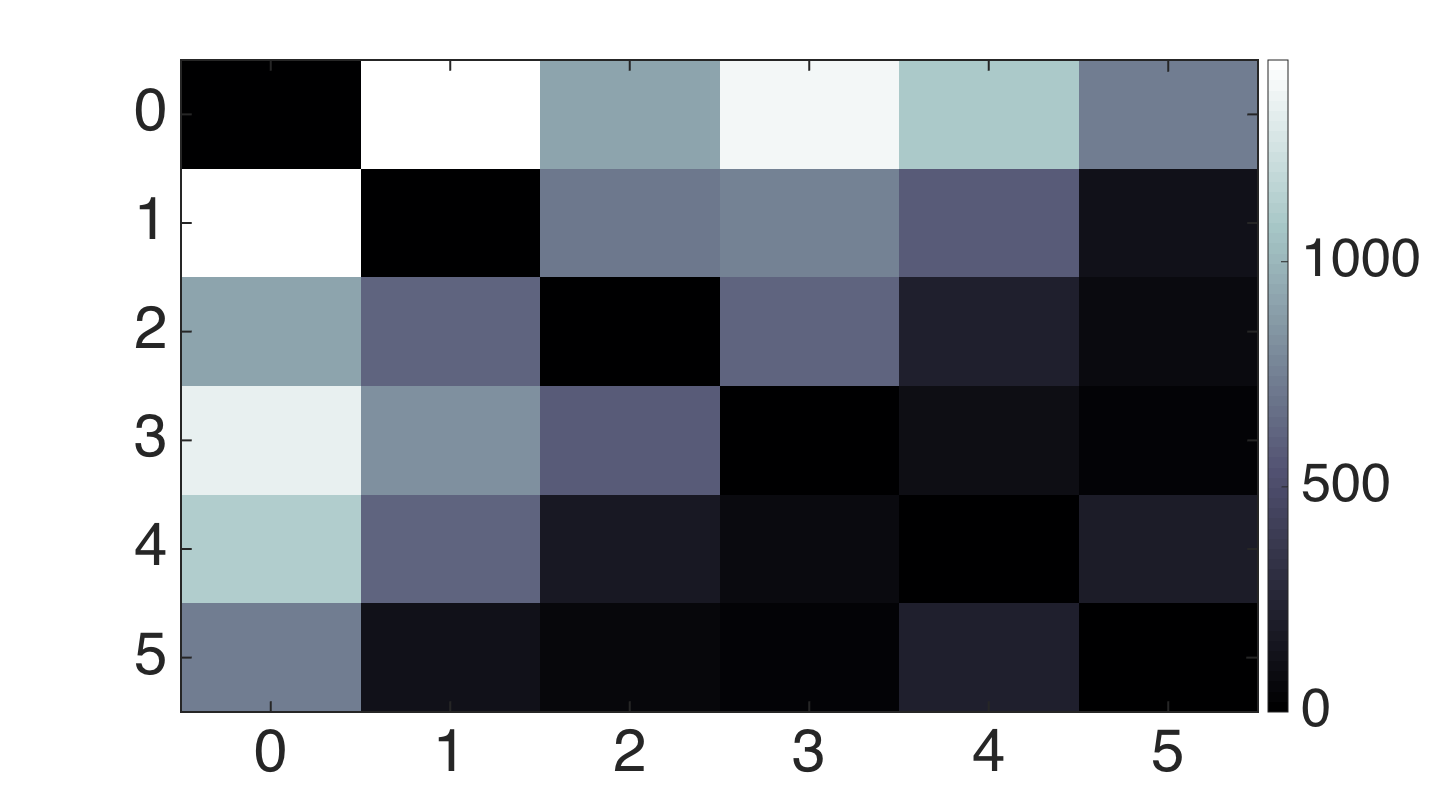
\includegraphics[width=1in,height= 0.7in]{figures/transdd.png}
             } 
               \hfill   
            \subfigure[FXS-F]{
            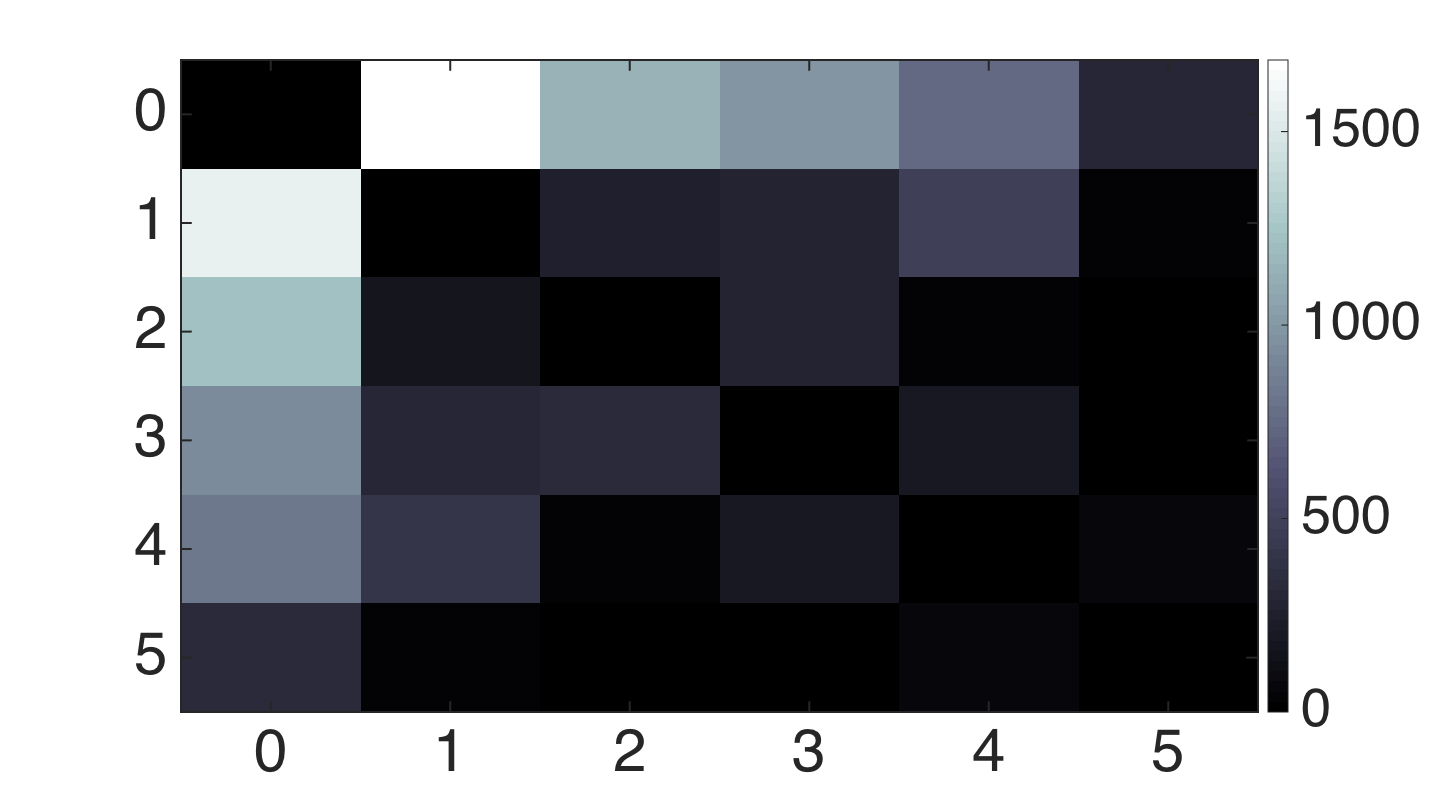
\includegraphics[width=1in,height= 0.7in]{figures/transfemale.png} 
            }
               \hfill
             \subfigure[FXS-M]{
            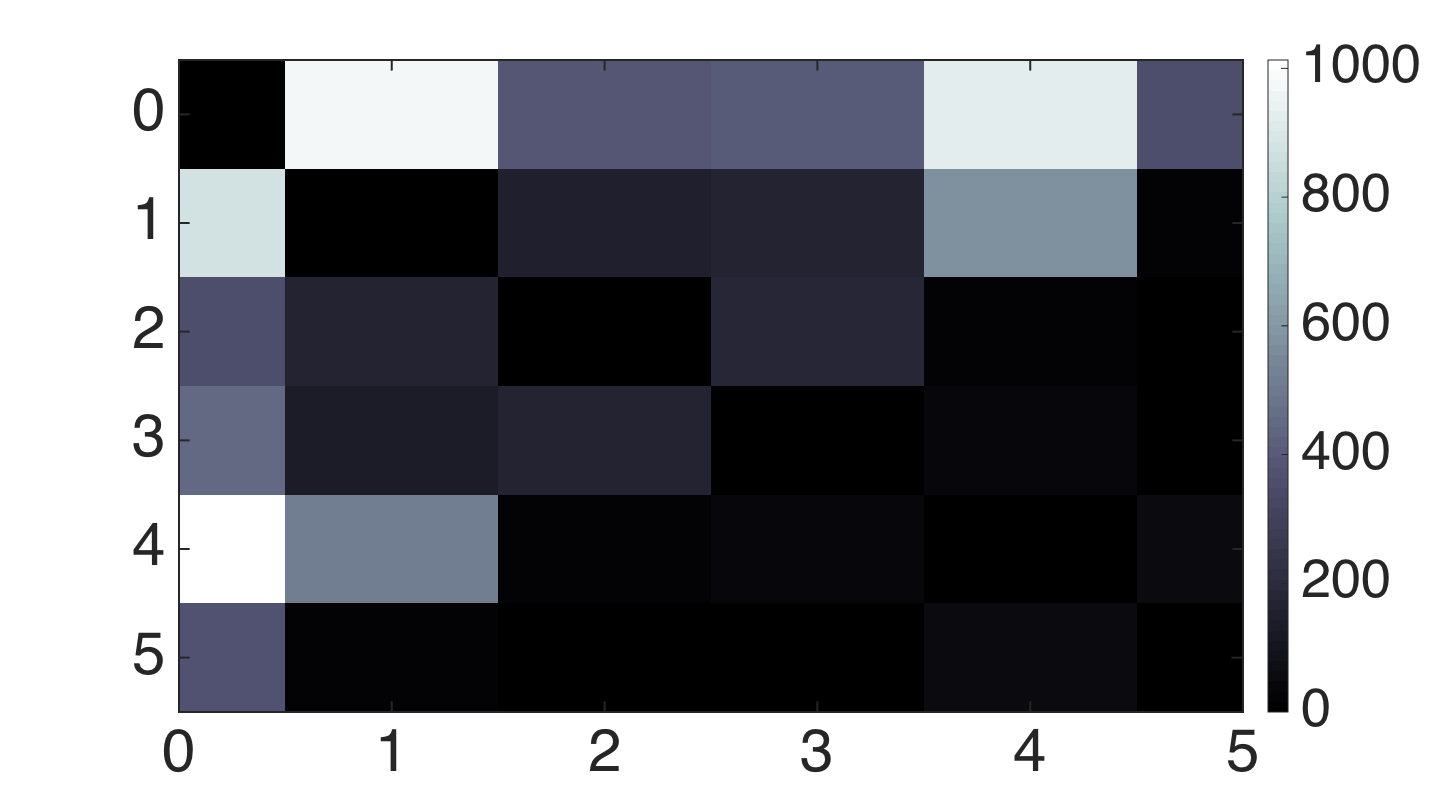
\includegraphics[width=1in,height= 0.7in]{figures/transmale.png} 
            }            
\caption{Matrix of attentional transitions for each disorder. Each square $[ij]$ represents the aggregated number of times participants of each group transitioned attention from state $i$ to state $j$.  The axes represent the different states: non-face (0), nose (1), eye-left (2), eye-right (3), mouth (4), and jaw (5).}
\label{fig:transitions}
\end{figure}

There is significant variance amongst individuals in the same group, making it challenging to classify between them. For example, Figure \ref{fig:sticky} shows time-series data of when individuals are glancing at the face of their interviewer or away from it. Note the varying sparsity of FXS males - some individuals glance at the face very frequently, whereas others may spend minutes without looking at it. FXS females exhibit similar sparsity amongst some individuals and much more consistent face-glancing amongst others. DD participants, on the other hand, tend to have a much higher frequency of glancing at the face, though a few participants also spend noticeable amounts of time looking away from it. 

\begin{figure}
       
       \subfigure[DD - Group]{
             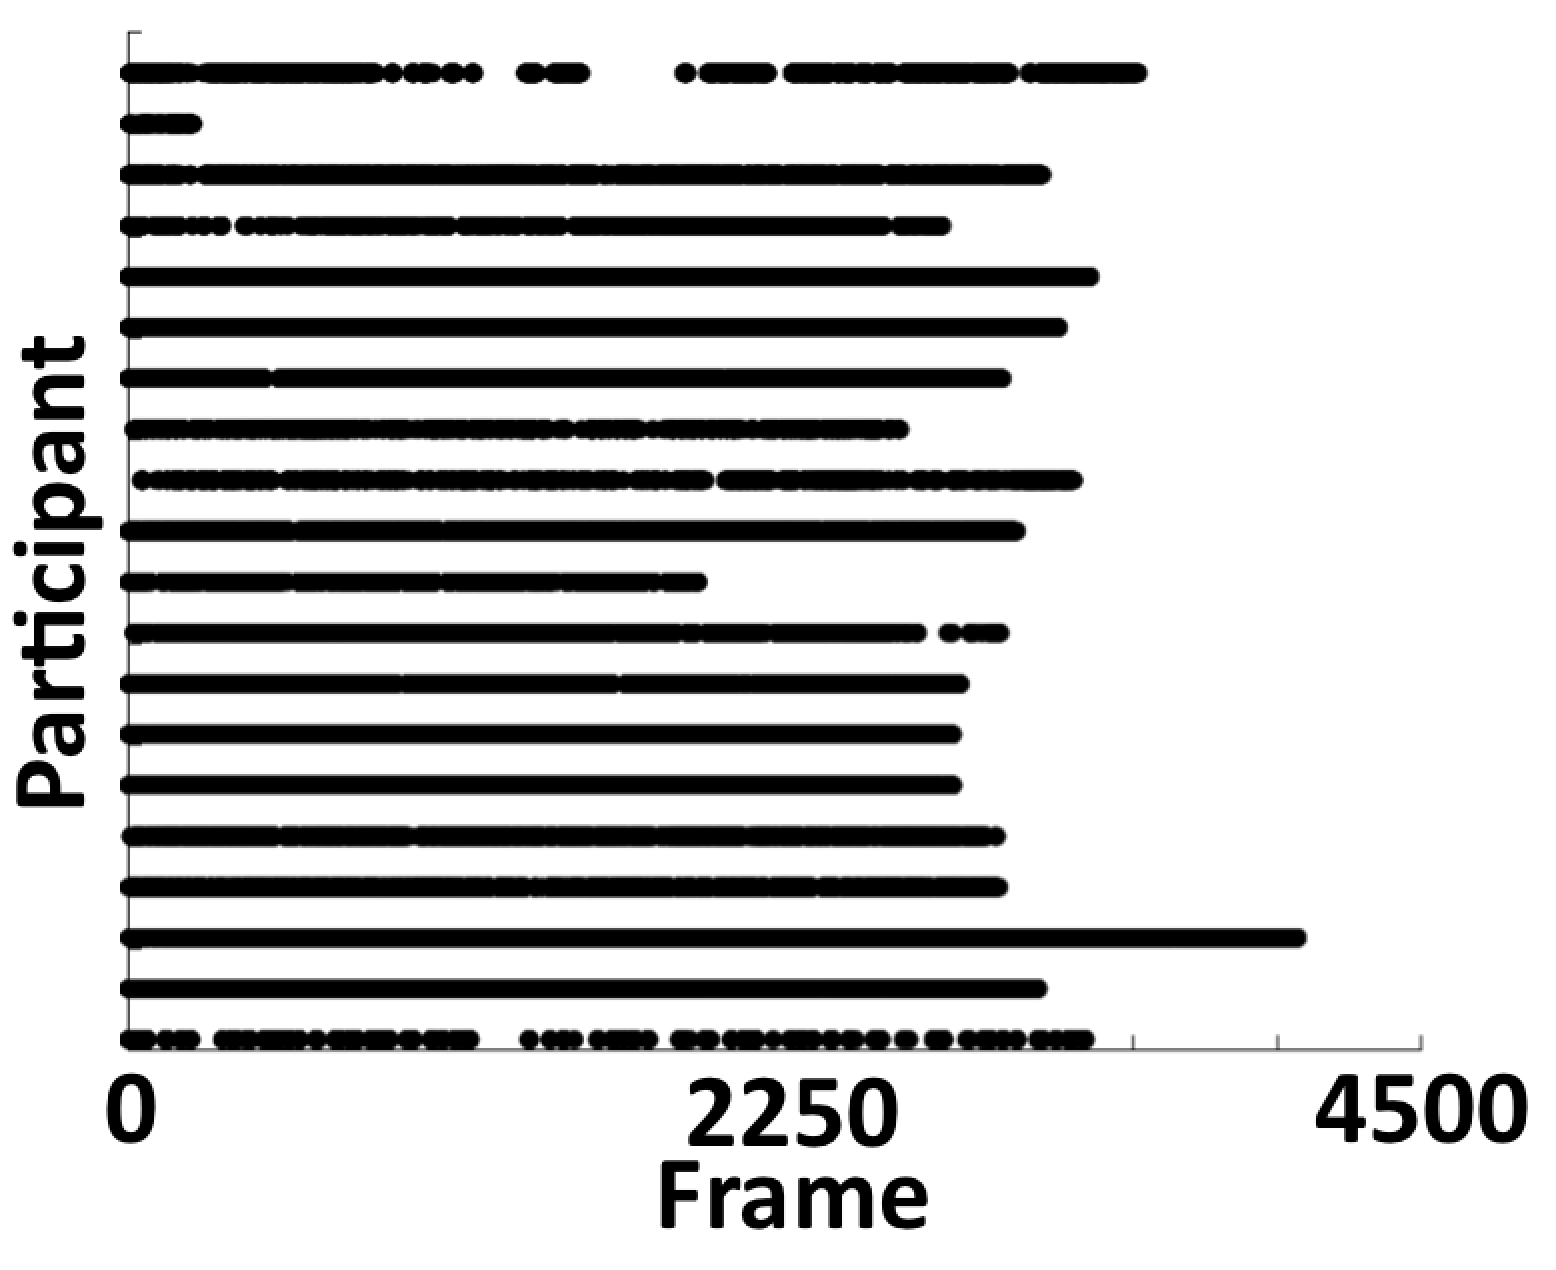
\includegraphics[width=0.22\textwidth]{figures/FXSF-face.png}
            }
            \hfill
          \subfigure[FXS Female]{
             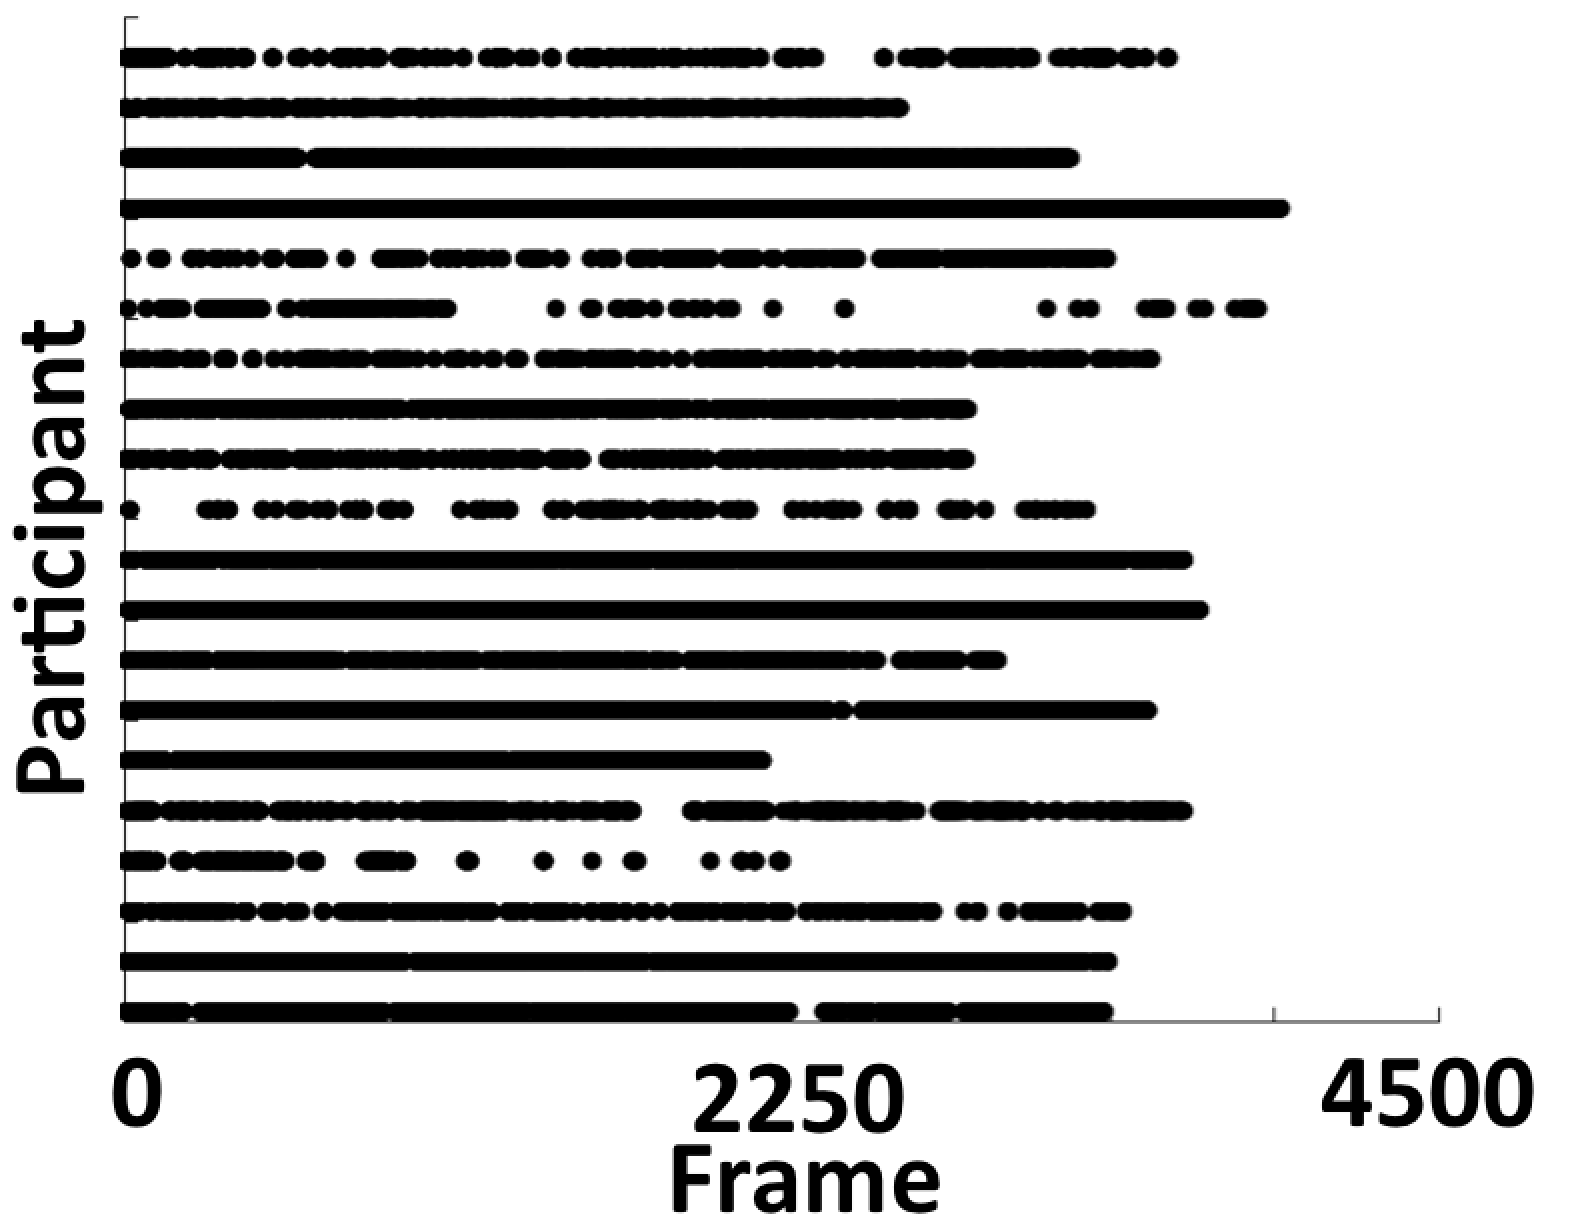
\includegraphics[width=0.22\textwidth]{figures/DD-face.png}
            }
            \hfill
            \centering
              \subfigure[FXS Male]{
             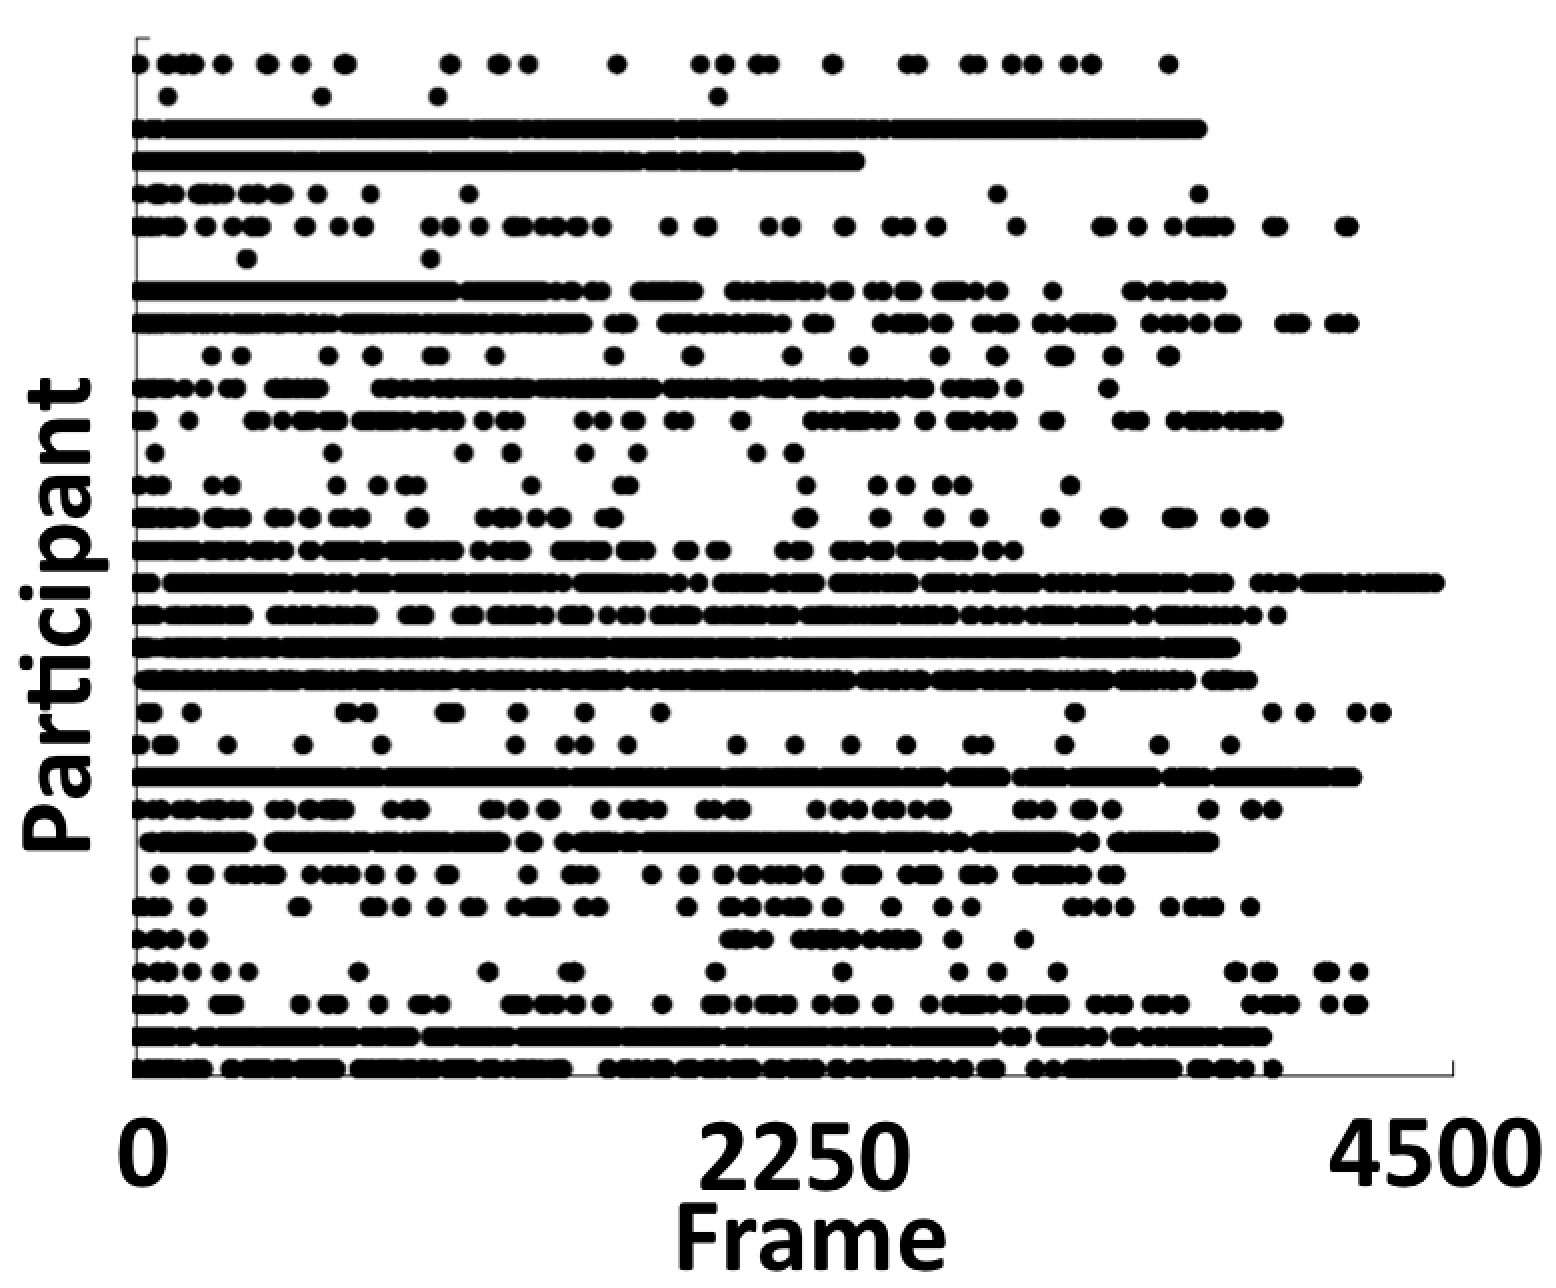
\includegraphics[width=0.22\textwidth]{figures/FXSM-face.png}
            }
        
         \caption{Temporal analysis of attention to face. X axis represents time in frames (in increments of 0.2 seconds). Y axis represents each participant. Black dot represent time points when the participant was looking at the interviewer's face. White space signifies that they were not.}
          \label{fig:sticky}
\end{figure}


\subsubsection{Approximate Entropy} 
 Approximate Entropy ($ApEn$) analysis provided a measure of how predictable a sequence is. The $ApEN$ of a signal is a value in $[0,1]$, where a higher entropy value indicates unpredictability of fluctuations in the signal, and a low value indicates a high degree of regularity. We employ ($ApEn$) analysis \cite{Restrepo:2014gs,entrophy} to further emphasize the similarity between DD and FXS-F signals and the difference between FXS-M and the other two. $ApEn$ measures the logarithmic likelihood that if two vectors $(q^{w}_{i}, q^{w}_{j})$ representing feature sequences of length $w$ are within a distance $R$, called the tolerance, in a w-dimensional space, then they remain within R in a $(w + 1)$-dimensional space when their length is extended by an extra feature. Greater (lesser) likelihood of remaining close produces smaller (larger) $ApEn$ values. To estimate $ApEn(R, m, N)$ for a length N feature sequence $Q={\bar{f}_1, \bar{f}_2, . . . , \bar{f}_{N}}$, given the parameters $w$ (window length), $\tau \in \mathbb{N}$ (subsampling coefficient), and $r \in \mathbb{R}^+$, we define the $w$-dimensional embedded vectors $q^{m}_{i}=[\bar{f}_{i}, \bar{f}_{i+\tau}, \bar{f}_{i+2\tau}, . . . , \bar{f}_{i+(m-1)\tau}]$, with $1 \leq i \leq N-(m-1)\tau$. 

We have measured the $ApEn$ of our 3 groups (DD, FXS-Female, FXS-Male). For each group $S_c$ we select 10 random participants (about 30,000 features $\bar{f}_i$). %$Q$ contains the vectors $u$ of features of $\sim$10 participants per group. The participants are chosen randomly. 
We parametrize $\tau=1$ to capture the entropy of the shortest period of time allowed by the data resolution (0.2 seconds). The tolerance parameter $r=0.1k$, for $k=1...30$ defines the tolerance $R = \text{std}(Q)r$. Figure \ref{fig:entropy}(a) depicts the $ApEn$ for $m=3$ while varying r. The FXS-M data is more stable than DD and FXS-F data, which share a similar entropy. 
\begin{figure}
        \subfigure[Tolerance Parameter]{
             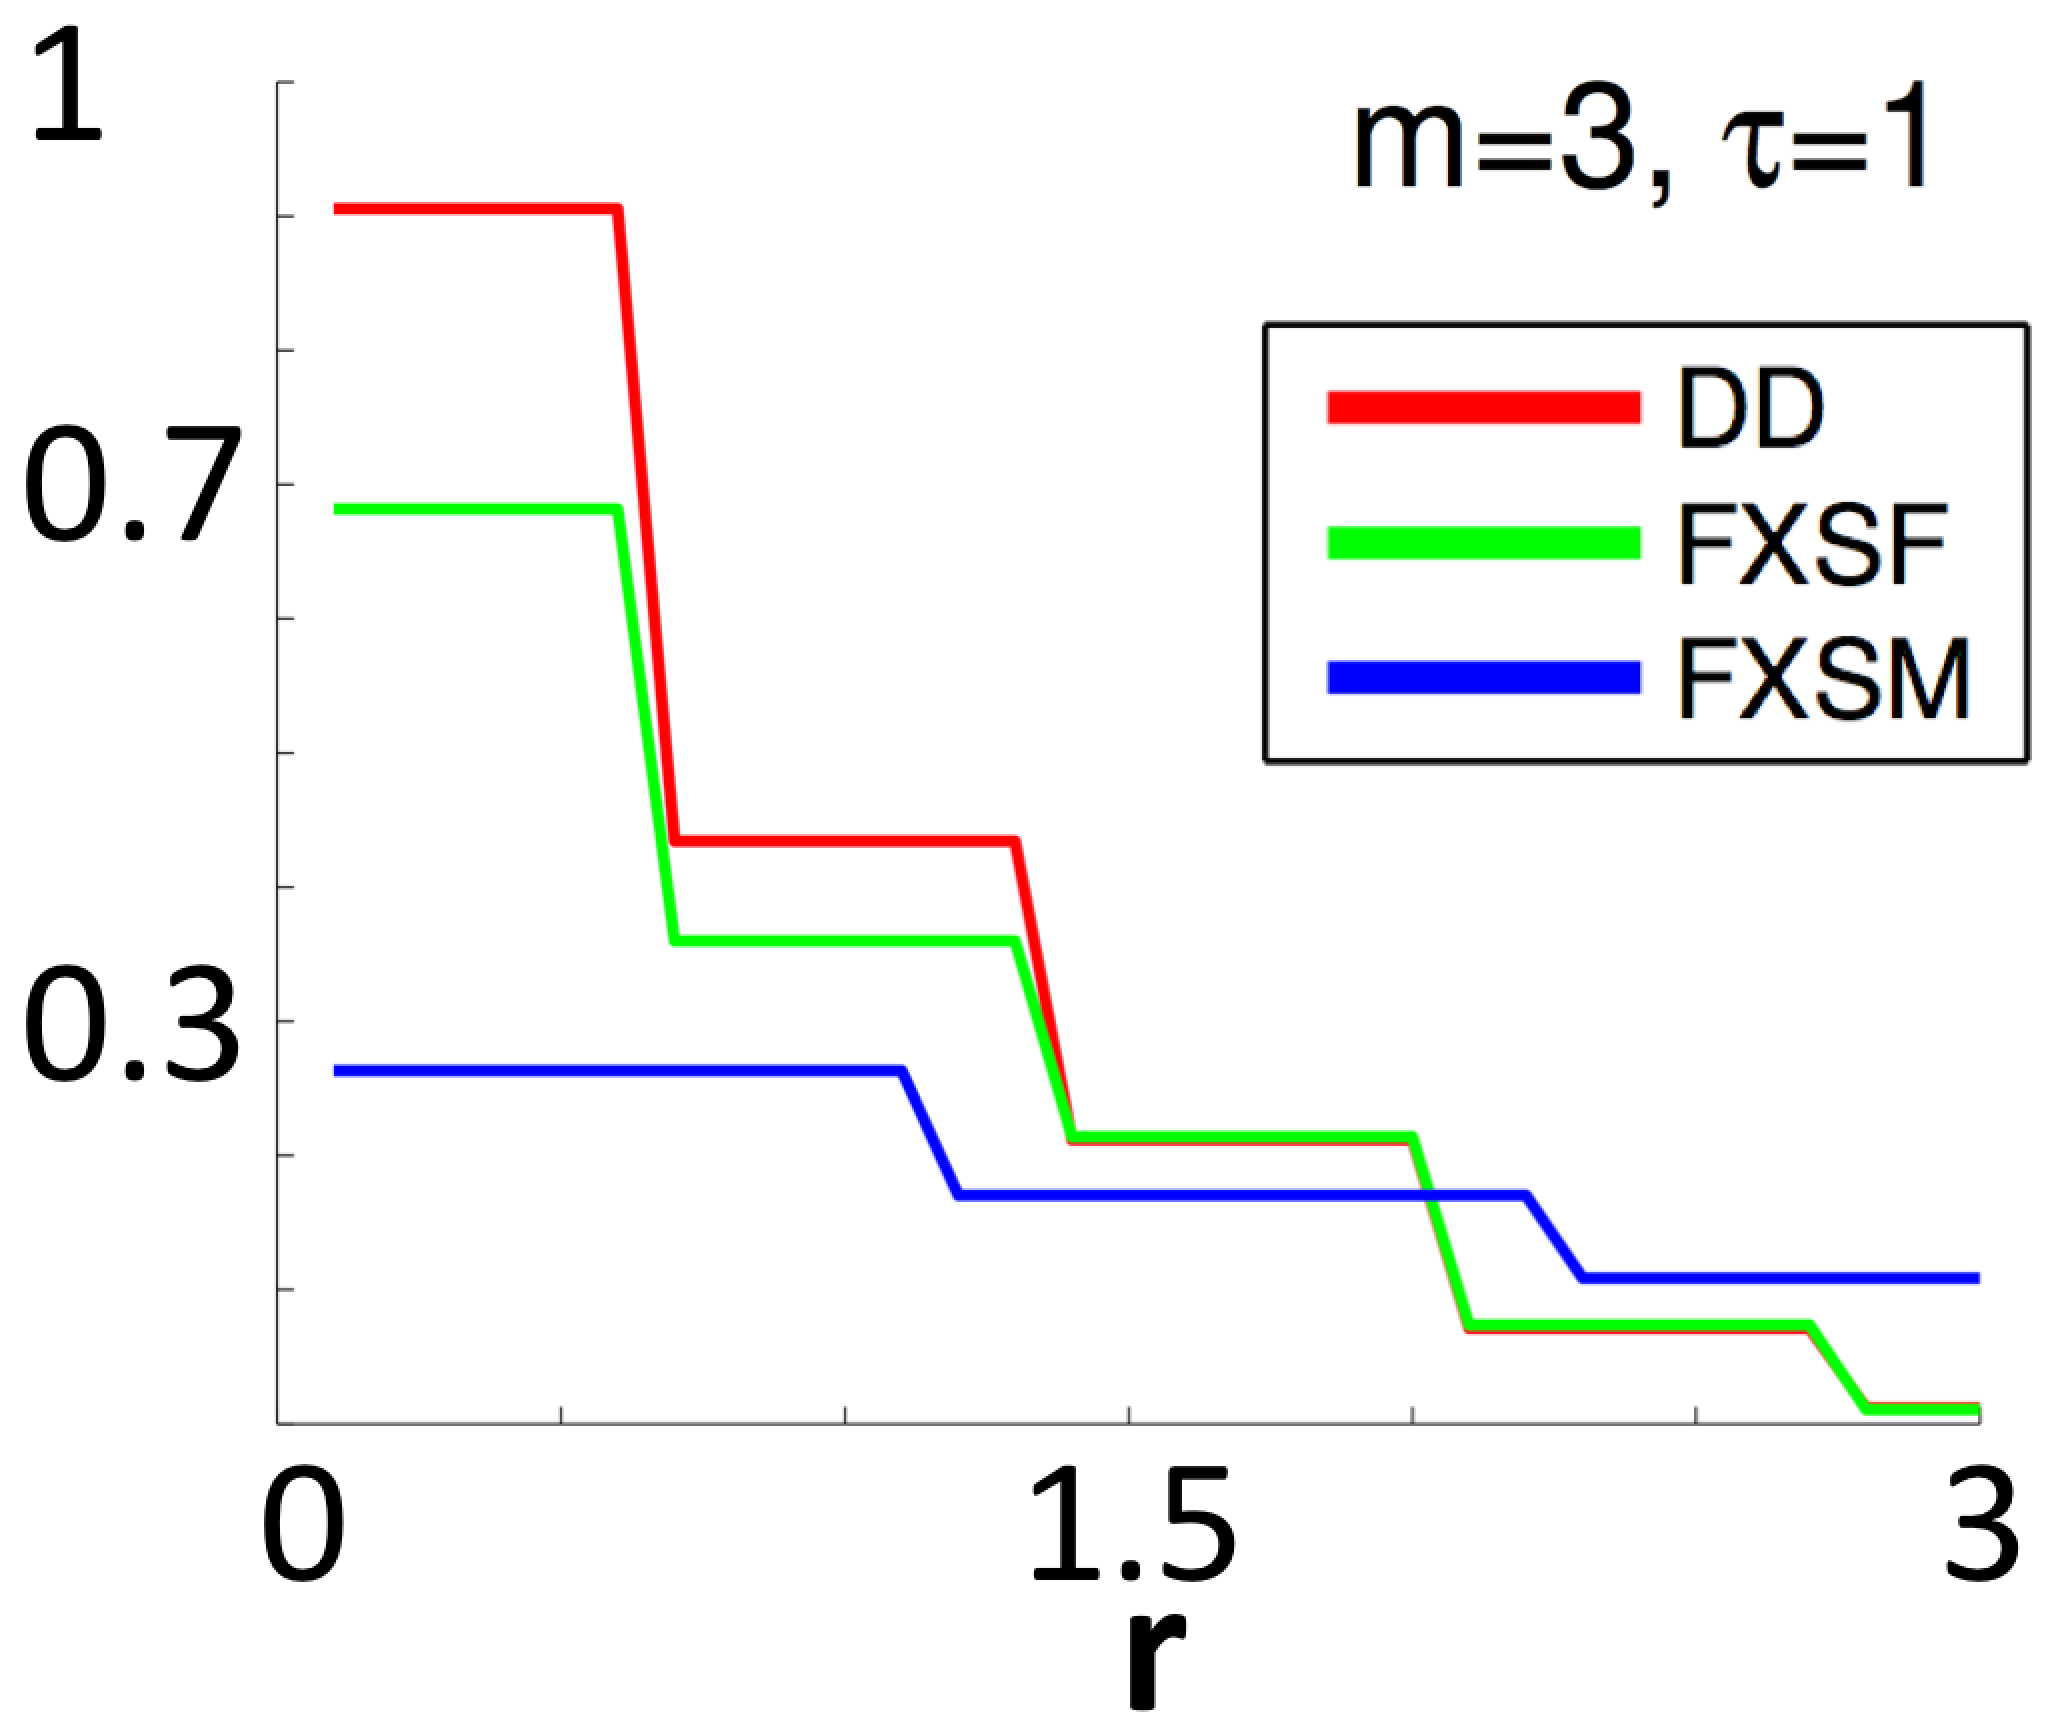
\includegraphics[width=0.2\textwidth]{figures/entropy-r.png}
        }
            \hfill
        \subfigure[Dimension]{
             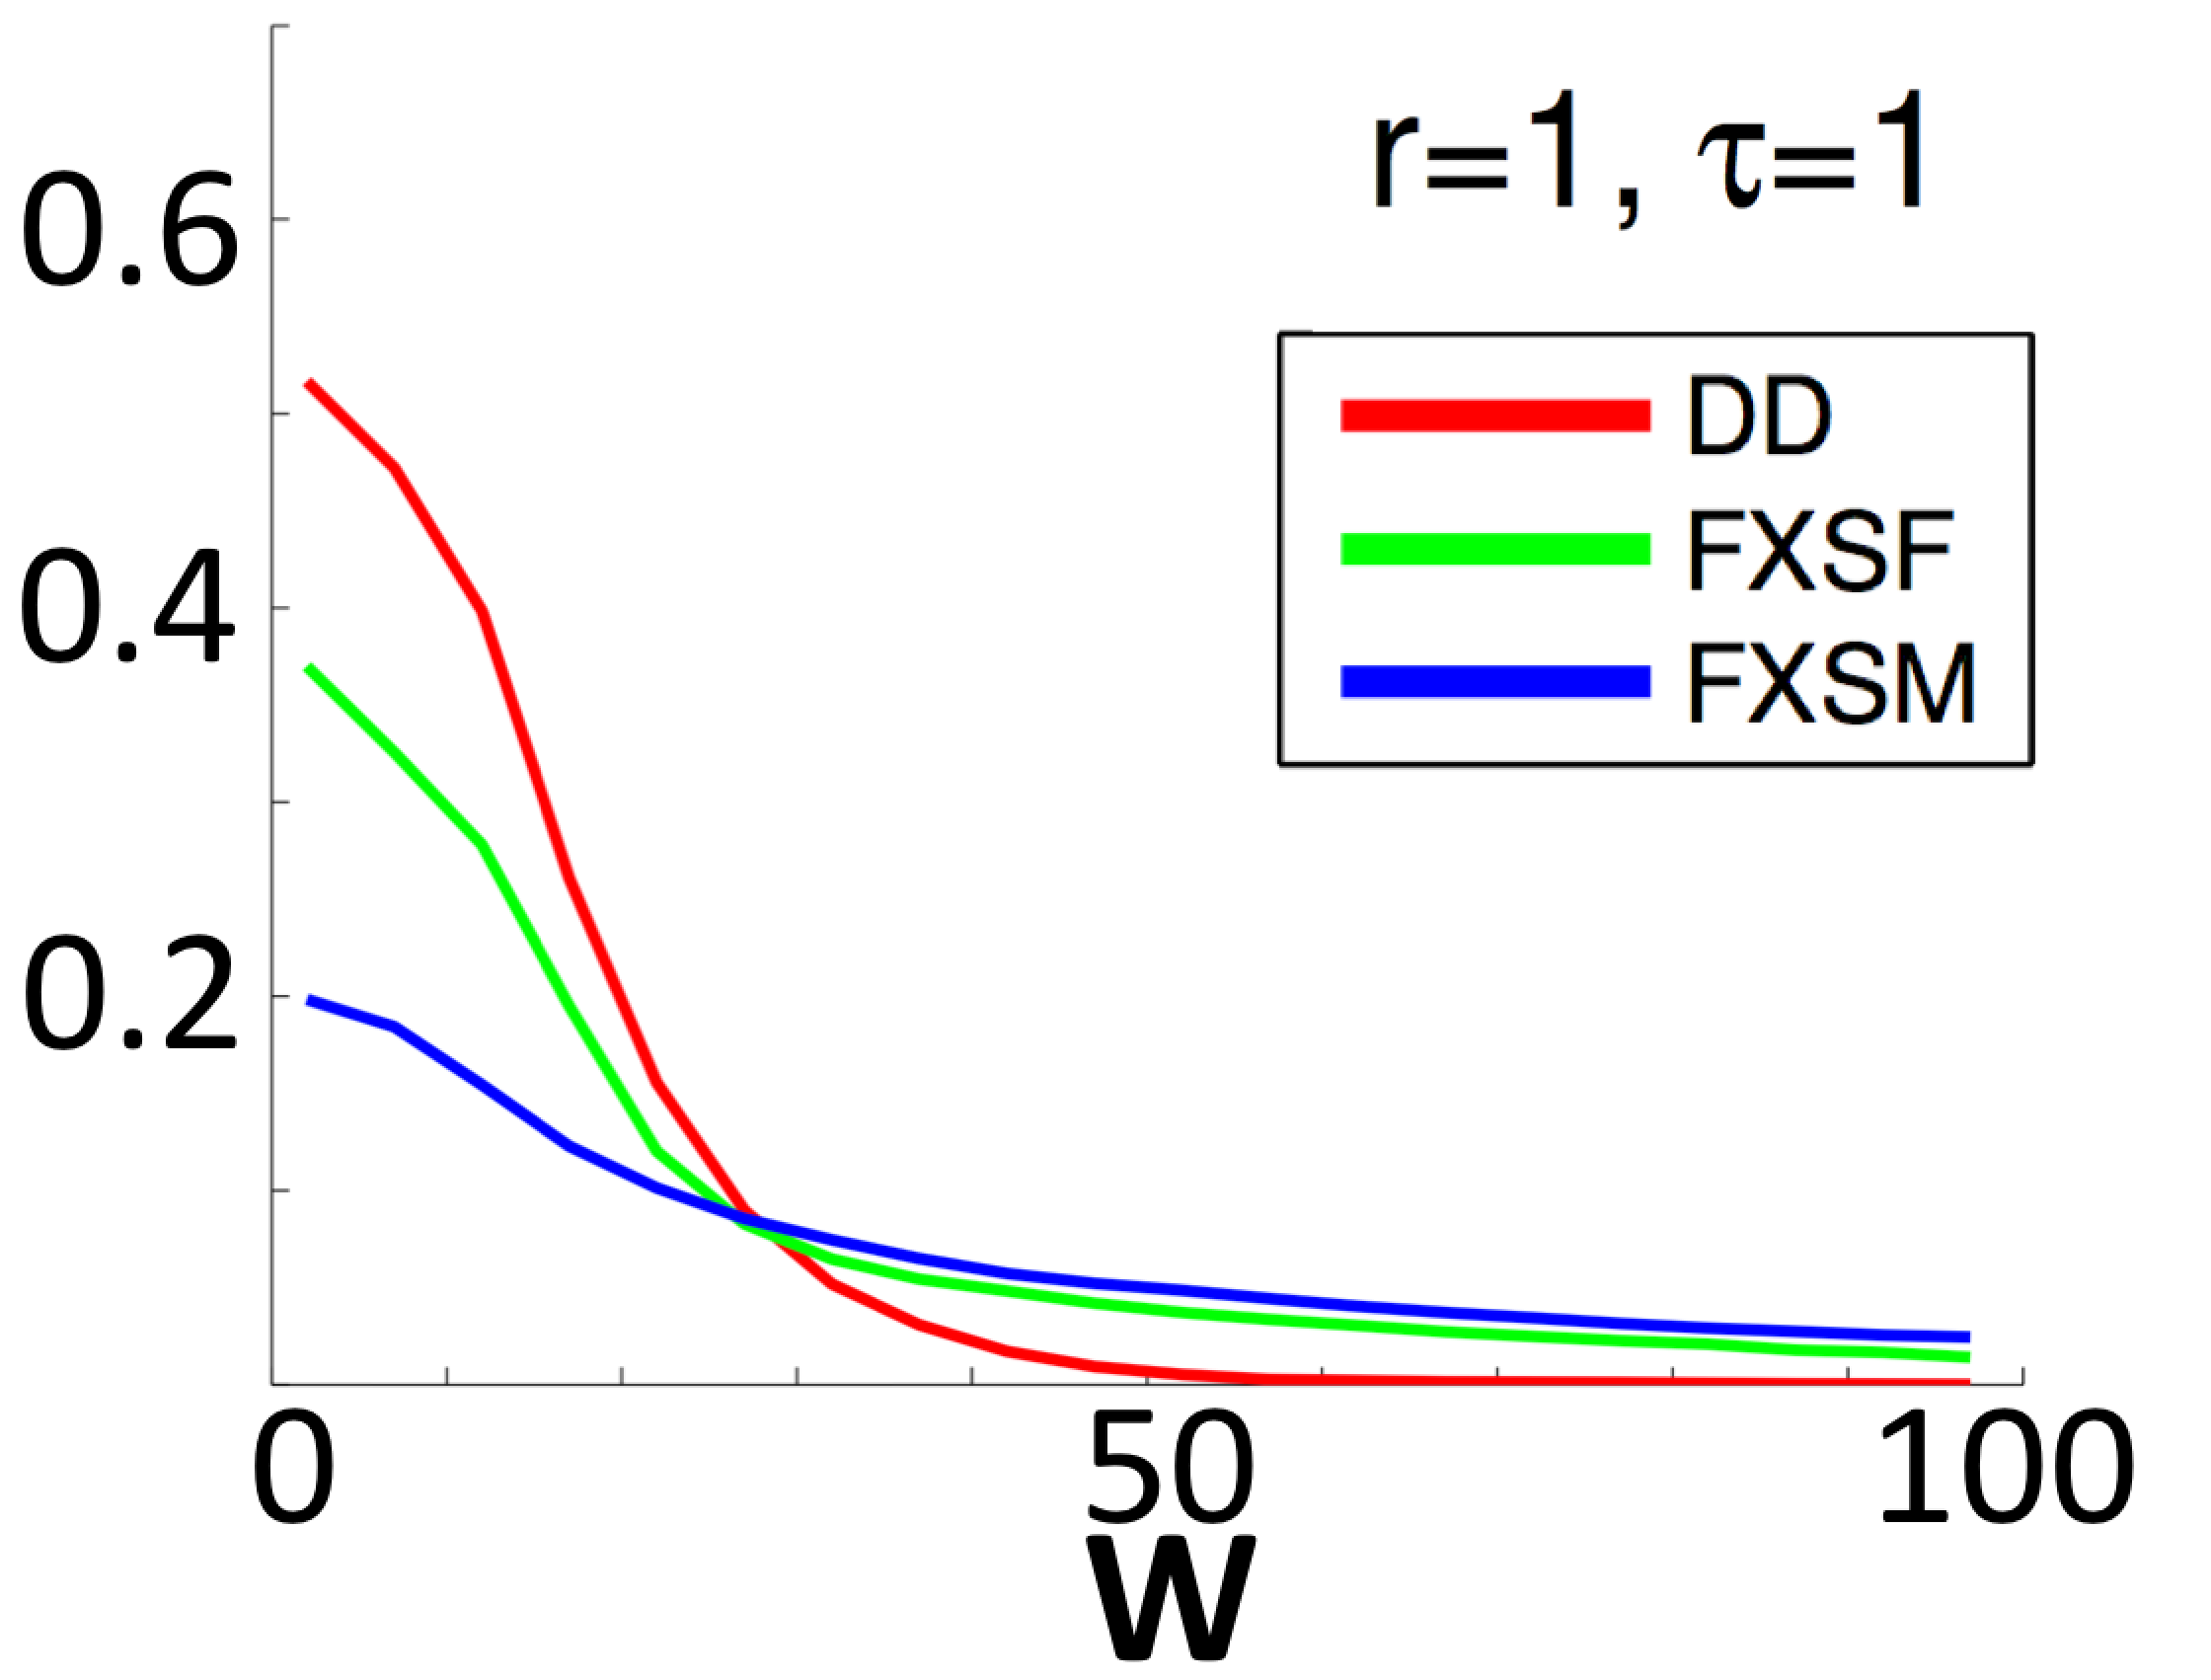
\includegraphics[width=0.2\textwidth]{figures/entropy-w.png}      }
       
        \caption{Analysis of the average $ApEN$ of the data for each participant class. X-axis represents (a) the tolerance parameter $r = R/std(Q)$, (b) the dimension parameter $w$.}
         \label{fig:entropy}
\end{figure}

Furthermore, we vary $w$ in order to understand the volatility of the signals from frame to frame. Figure \ref{fig:entropy}(b) depicts such an analysis. Here the parameter $R$ is fixed to $R=\text{std}(Q)$. We see that FXS-M participants, on average, show the most stable decay for small $m$ while FXS-F and DD share a similar decay rate. Simultaneously we see in Figure \ref{fig:individual_entropy} that there is great variance amongst individuals of each population. This is taken using about 6.6 minutes of data (2000 features) from each participant. We compute the $ApEn$ by fixing $\tau=1$, $r=1$ and varying $w$. 
\begin{figure}[b]
        \centering
        \subfigure[DD]{
             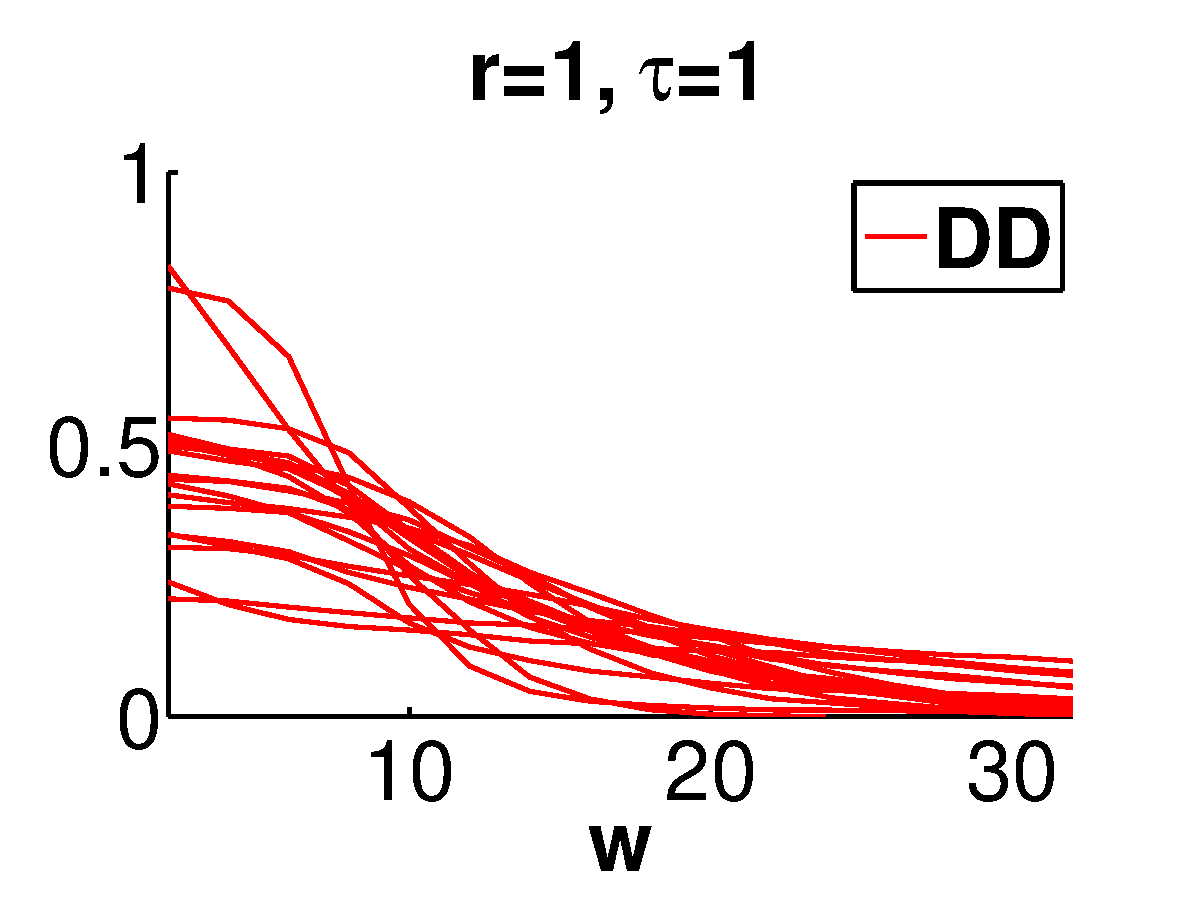
\includegraphics[width=0.2\textwidth]{figures/DDen}
        }
            \hfill
        \subfigure[FXS-F]{
             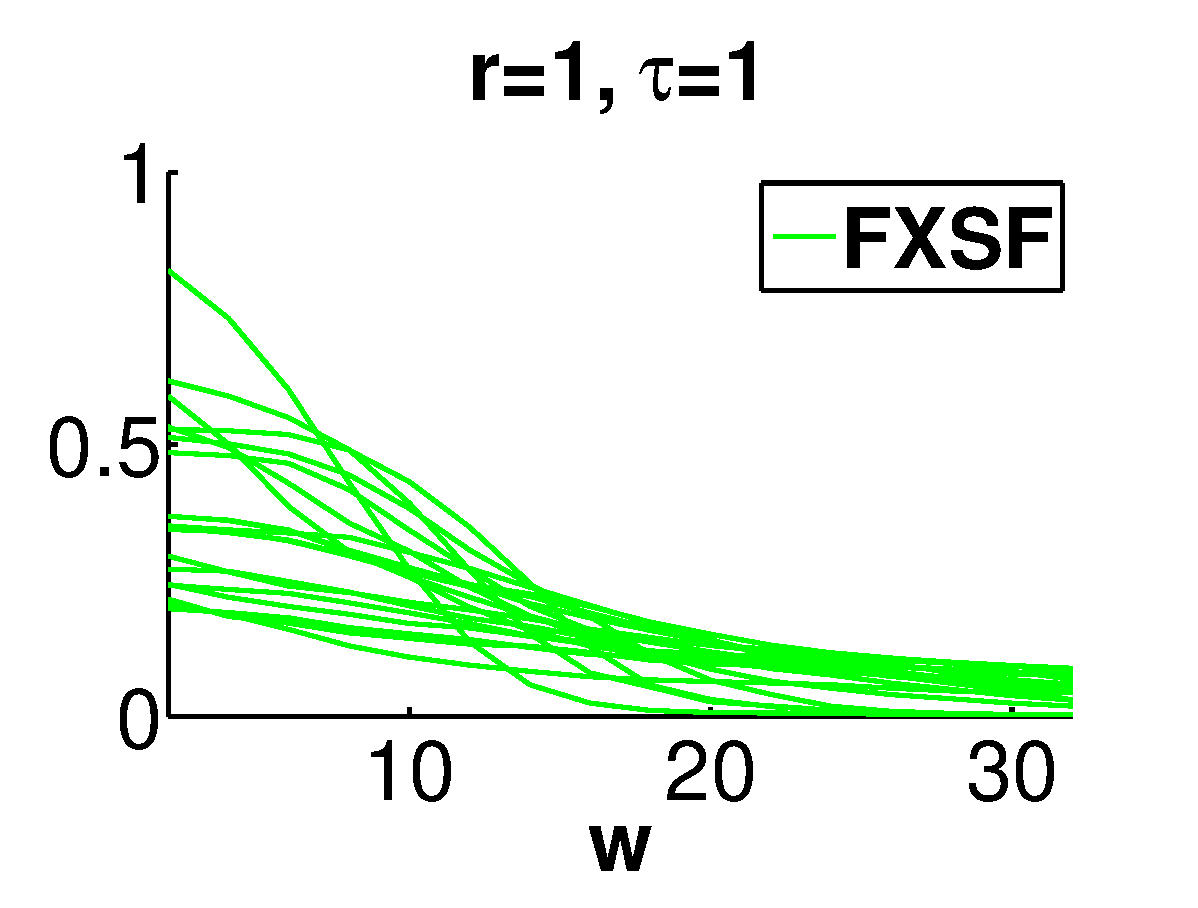
\includegraphics[width=0.2\textwidth]{figures/FXFen}      }
             \hfill
         \centering
         \subfigure[FXS-M]{
             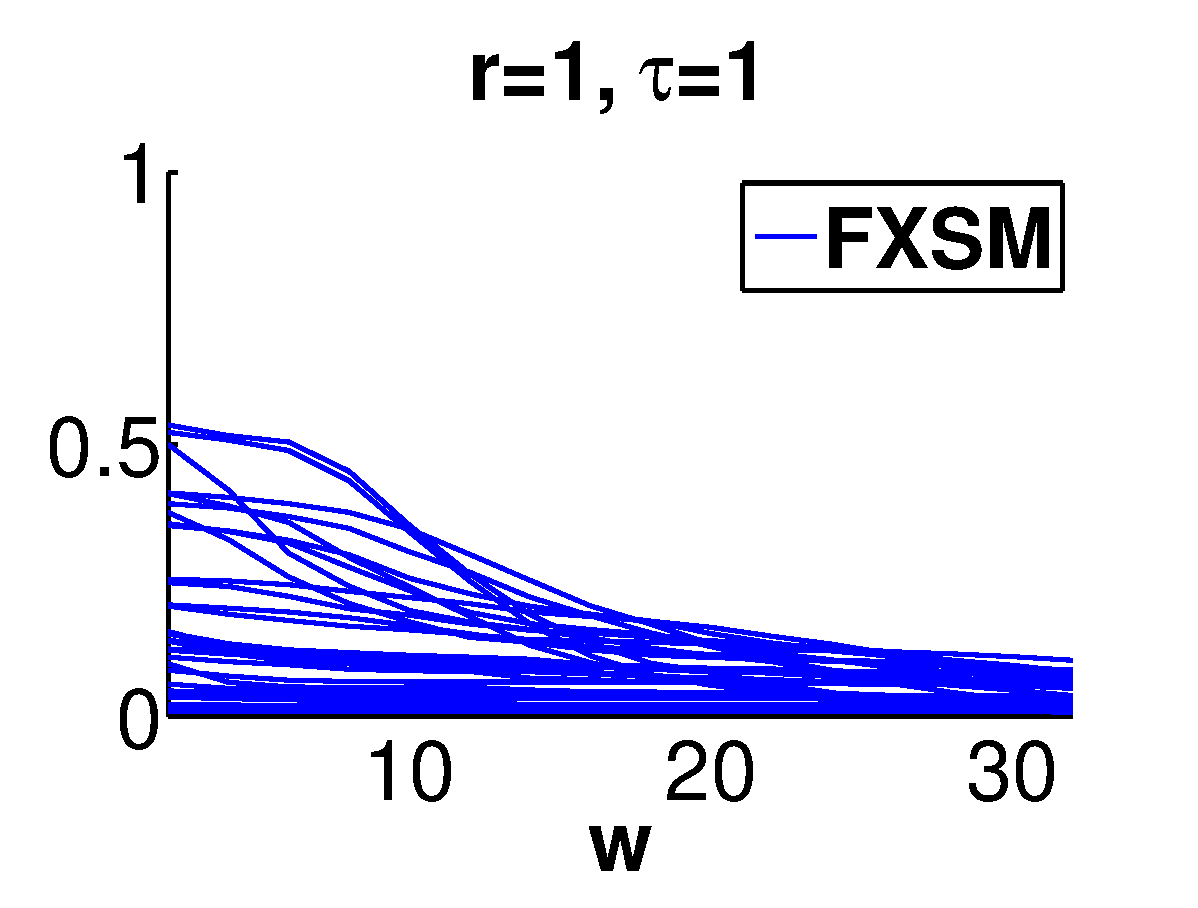
\includegraphics[width=0.2\textwidth]{figures/FXMen}}
        \caption{Analysis of the $ApEn$ of the data per individual varying the dimension parameter $w$. Y-axis is $ApEn$ and X-axis varies $w$. Each line represents one participant's data.}
        \label{fig:individual_entropy}
\end{figure}


%%%%% SECTION: CLASSIFICATION AND EVALUATION
\section{Training of Classifiers}
\label{sec:classification}

The goal of this work is to create an end-to-end system for classification of mental disorders from raw visual information. So far we built features that capture social attentional information and analyzed their temporal structure. We need to construct methods capable of utilizing these features to predict the mental disorder of a participant. Given the novelty of this dataset, the key challenge is to find methods that can tackle the intrinsic structure of the data and discern between participants. We propose a one-dimensional convolutional neural network designed to work with state-vectors. We train other models for comparison against this one.

We form an input data matrix and label vector by choosing a window length $w$ and a step size $s$ and converting the feature sequence of our entire dataset, $Q=[f_1^1, f_2^1,...,f_{T_N-1}^N,f_{T_N}^N]$ into the $m \times w$ matrix
\begin{equation}
X = \begin{bmatrix}
f_1^1 & f_2^1  & ...  & f_w^1 \\ 
f_{1+s}^1 & f_{2+s}^1  & ...  & f_{w+s}^1 \\ 
\vdots  & \ddots  &  & \vdots  \\ 
f_{T_N-w}^N & f_{T_N-w + 1}^N  & ... & f_{T_N}^N
\end{bmatrix}
\end{equation}
With corresponding labels vector $Y=[Y_1,...Y_m]$ where the label $Y_i$ is either 0 or 1 depending on the disorder of the patient whose features were used to form row $i$. 

\subsection{State Vector CNN}
\label{sec:CNN}
Convolutional neural networks are good models for representing data with highly correlated features (e.g.  speech and image \cite{Krizhevsky:2012wl, hamidss, Bouvrie:2006vb,lecun}). Our feature sequences fit this data profile. We propose a one-dimensional convolutional neural network approach that can exploit the local-temporal relationship between state vectors. Our state vector CNN (S-CNN) works with states represented by sparse vectors. %It takes as inputs sub-sequences of features $q=[f_i,...f_{i+w}]$ of length $w$ where each sub-sequence is labeled 0 or 1.

%\subsubsection{Network Configuration}

Figure \ref{fig:conv} depicts the architecture of our S-CNN. It is composed of one hidden layer of $U=6$ convolutional units followed by point-wise sigmoidal nonlinearities. The feature vectors computed across the units are concatenated and fed to an output layer composed of an affinity followed by another sigmoid function.

Recalling the state-vector representation of the features $f=<x_1,x_2,...x_6 >$ where $x_i \in \{0,1\}$ we now represent the input rows $q$ of $X$ to the CNN in this state-vector form $q=[x_i,...,x_{i+l}]$ where $l$ is the new dimensionality of the input data under this extension.

We choose the kernel size $k$ of the hidden units and stride $s$ to be a multiple of $\tau=6$, the length of a feature $f$, to avoid splitting state-vectors between filter steps. We parametrize $s=6$ and $k=24$ (i.e. ~ 0.8 sec. of video). The S-CNN has an output layer composed of a single unit which outputs a continuous value in the range $[0,1]$. We threshold this value at $0.5$ for classification. 

\begin{figure}
       \centering
       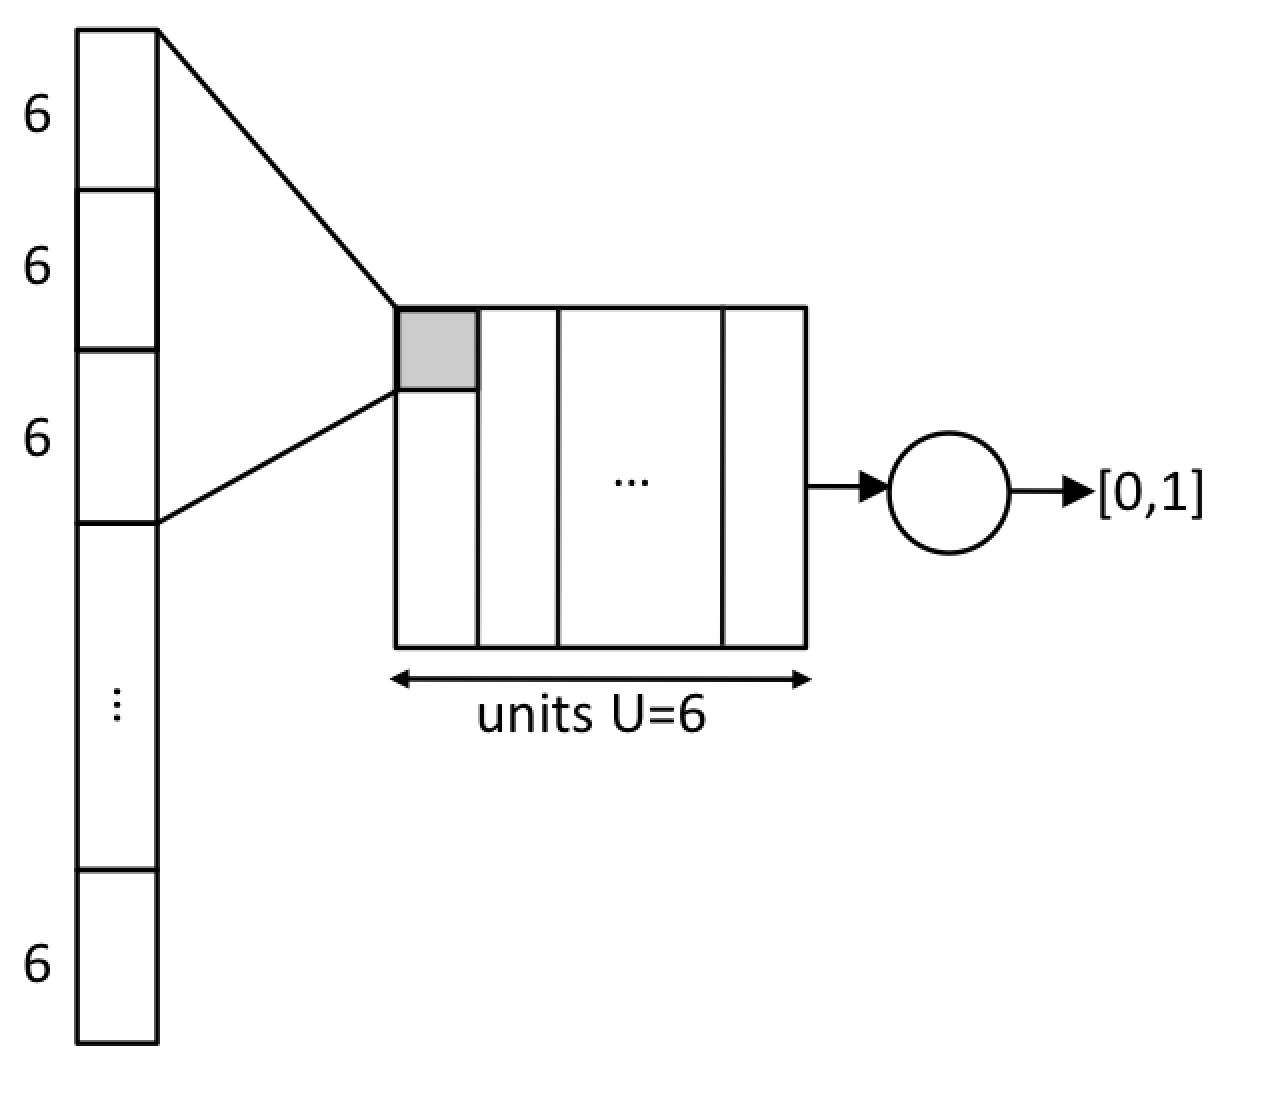
\includegraphics[width=0.3\textwidth]{figures/network.png}  
        \caption{Convolutional Neural Network Design. The input is a binary vector representing a sequence of features. The CNN is composed of a single hidden layer and an output layer. The filters are chosen to be an integer multiple of 6, the length of the state vectors. The output is a sigmoid, thresholded to 0.5 for classification}
              \label{fig:conv}
\end{figure}

%\subsubsection{Learning algorithm}

In the convolutional layer we have that the activation map of a unit is given by a vector $\textbf{a}$ whose $j^{\text{th}}$ entry is given by:
\begin{equation}
a_{j} = \sigma \left (\sum_{i=1}^{k}{w_{i}^{(1)} \: x_{i + (j-1)\:s}} \right )
\end{equation}

Where $\sigma$ is the sigmoid function and $w_i^{(1)}$ are input weights. The $U$ activation maps are concatenated into a single vector $\textbf{v}$. The output of the S-CNN is then given by:
\begin{equation}
y = \sigma \left (\textbf{v}^T \textbf{w}^{(2)} \right )
\end{equation}

%% Commented %%
\begin{comment}
To compute the pre-nonlinearity input to a unit in the hidden layer, we sum up the contributions (weighted by the filter components $w$) from the input. The $j^{th}$ convolution of any hidden unit is computed as:
\begin{equation}
o_{j} = \sum_{i=1}^{k}{w_{i} \: x_{i + (j-1)\:s}}
\end{equation}
Where $k$ is the unit kernel size and $s$ is the stride. The value $s$ must be multiple of $\tau$ to avoid convolving mistaken sparse sub-representations of a feature $f$. 
Then the convolutional layer applies its non linearity. 
\begin{equation}
a_{j} = \sigma(o_{j})
\end{equation}
Where, $\sigma$ is the sigmoid function and $\tau=6$.
\end{comment}
%% End Commented %%

The S-CNN is trained with backpropagation using stochastic gradient descent with momentum and a learning rate of 0.05. 

%% Commented backdrop stuff %%
\begin{comment}
The gradients $\delta$ of the hidden layer units are computed to update the layer weights. 
 
\begin{equation}
\delta_{j} = \delta v_{j} * a_{j} * (1-a_{j})
\end{equation}
where $a_j$ is the $j^{th}$ element of the unit's feature map, and $\delta v_j$ is the error gradient of the output layer. The weight gradients computation in the hidden unit considers the structure of the sparse vectors. For a convolutional unit the weight $i$ is updated as follows:

\begin{equation}
\triangledown w_{i} = \sum_{q}^{l} \sum_{t=1}^{n} \:\: \delta_{t} \:\:x_q \:\:\bold{1}(mod (q,\tau) = i)
\end{equation}
\begin{equation}
\delta v_i = w^{out}_{i}*\delta^{out}
\end{equation}
\begin{equation}
\delta^{out} = y \: (1-y) \: (y-\hat{y})
\end{equation}

where $l$ is the number of the input values $x_{\{1...l\}}$. The indicator function $\bold{1}(\hat x)$=$1$ for $x_{q}$'s that were weighted by $w_{i}$ that contribute to calculate $a_j$ in the forward pass. The values  $\delta^{out}$ and $\delta v_i$ are the gradients of the output layer, and $y$ and $\hat{y}$ are the predicted and expected output values. 

We use stochastic gradient descent to update the weights, where the learning rate is $0.05$. 
\end{comment}
%% End Comment %%

\subsection {Other Classifiers}
We train support vector machines (SVMs), Naive Bayes (NB) classifiers, and Hidden Markov Models (HMMs). 

We train SVMs using a chi-Squared kernel function to account for long sub-sequences of features with little variation (i.e. sequences with many 0's). 

Seeking an optimal window length for classification, we train a series of classifiers and and vary the window size from 1 feature (0.2 sec) up to 900 (3 minutes). We find small variance in classification error for windows up to 50 sec (= 250 features), and observe a similar result when trying other classifiers. This window sweep is shown in Figure \ref{fig:window_lengths}.

For comparison with traditional temporal classifiers, we train a two-hidden-state HMM with six possible emissions (corresponding to binary classification with vectors of six states). For the HMM classifier we take $Q=[f_1^1, f_2^1,...,f_{T_N-1}^N,f_{T_N}^N]$ and $Y=[b^1, b^1, ...,b^N]$, where $b^i \in {0,1}$ are the labels of the two mental disorders considered and correspond to the two states of the HMM. We divide both $Q$ and $Y$ into non-overlapping, contiguous sub-sequences of length $w$ and shuffle them to form the HMM emission sequence $Q^{s}$ and state sequence $Y^s$. We take a training set of this data and first estimate the transmission and emission probabilities of an HMM, and then use these probabilities to predict the HMM state of a testing set. 

%\begin{comment}
\begin{figure}[h]
        \centering
  
        \subfigure[DD vs FXS Female]{
             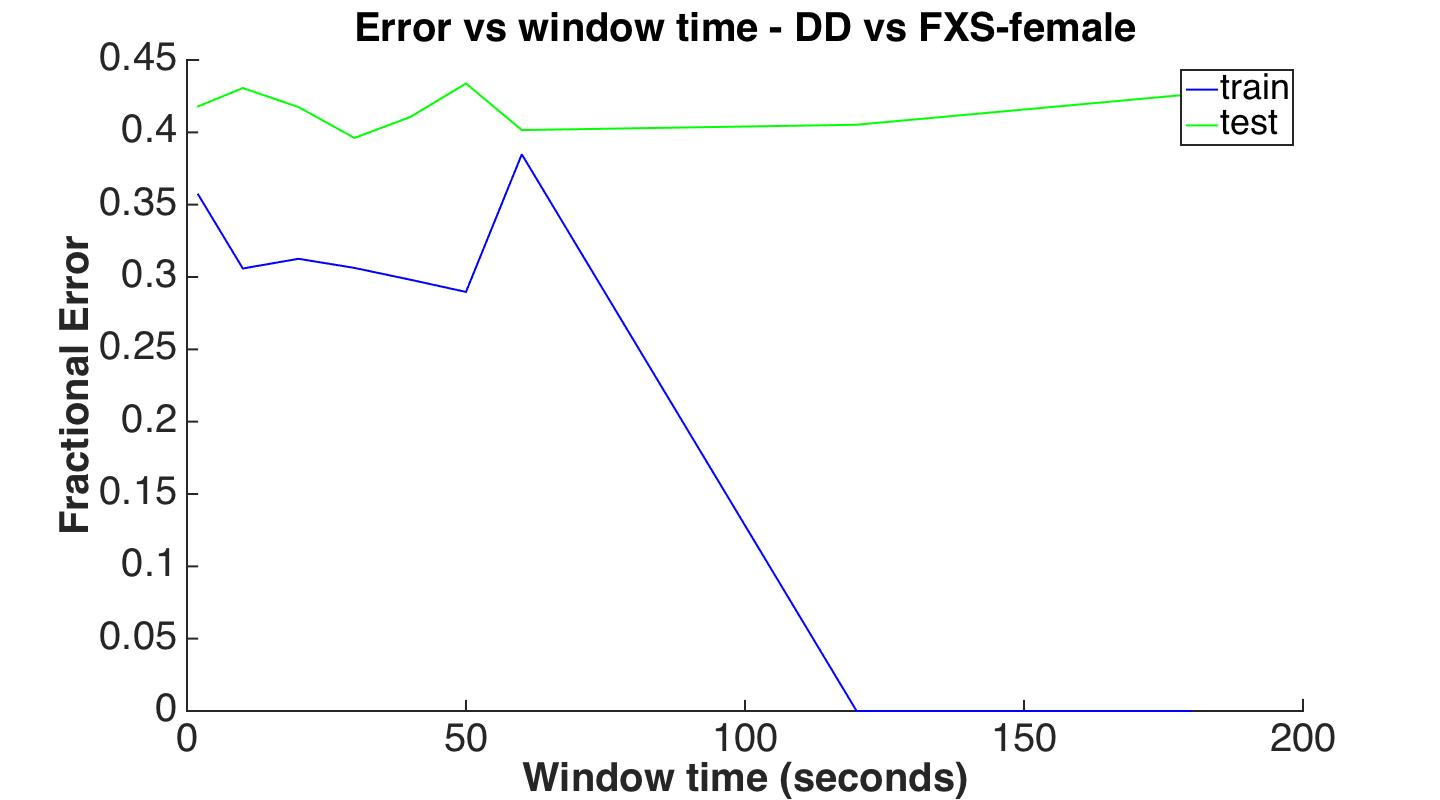
\includegraphics[width=0.25\textwidth]{figures/Temporal-DDvsFXSfemale-SVM}
        }
            \hfill
       \subfigure[DD vs FXS Male]{
             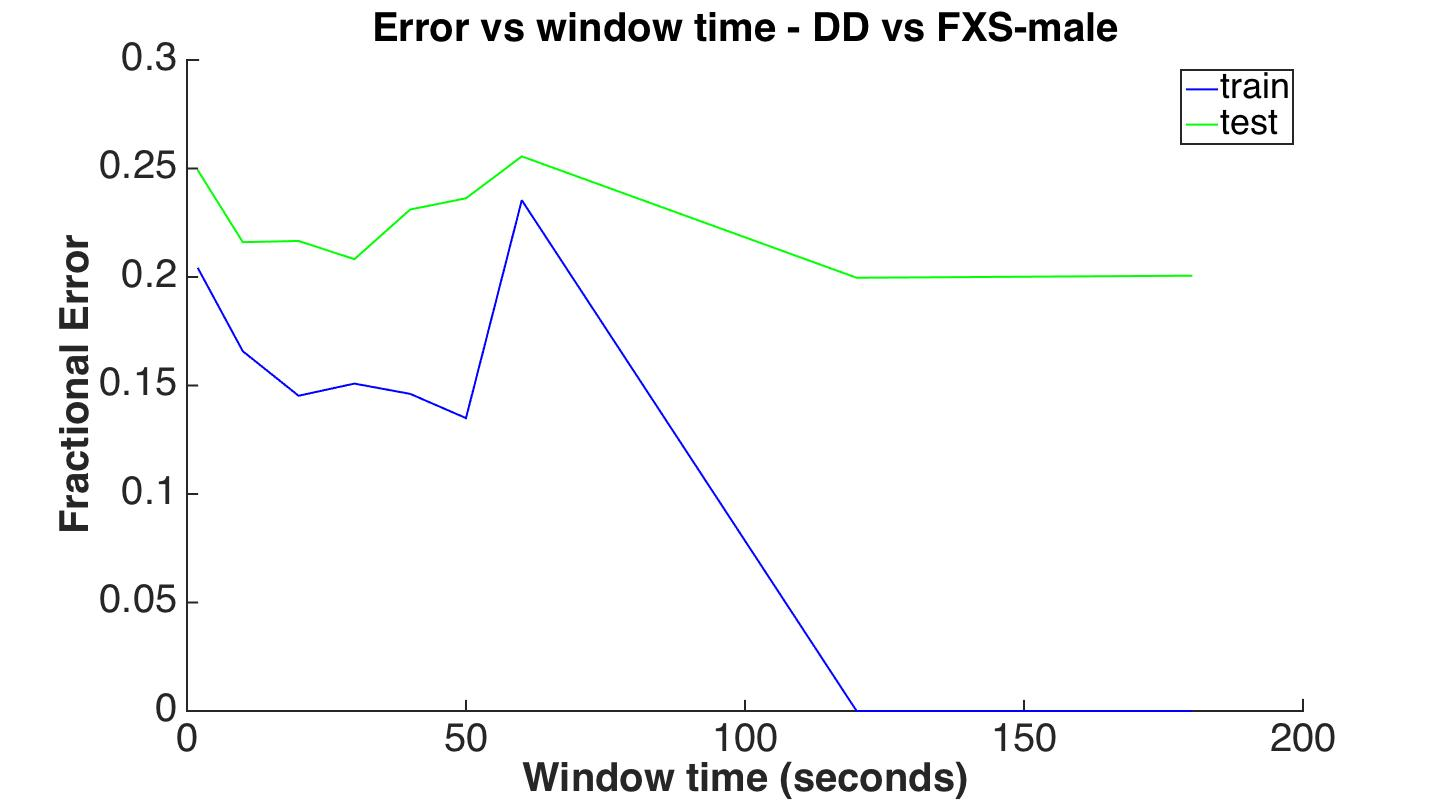
\includegraphics[width=0.25\textwidth]{figures/Temporal-DDvsFXSmale-SVM.jpg}
       }        \caption{Analysis of SVM classifier training and testing error as a function of time window  (in seconds) for pair-wise classifiers. One second of time corresponds to 5 features.}
        \label{fig:window_lengths}
\end{figure}
%\end{comment}

%As shown in Figure \ref{fig:window_lengths}, we trained a number of SVMs with varying window lengths and observed the training and testing errors. SVMs average training and testing error (over multiple folds) from small time windows of 2 seconds up to mid-size windows of 50 seconds changes very little. For longer time windows we see a characteristic spike in the training error followed by significant over-fitting for larger windows of time. 


%As can be seen from the plots of Figure \ref{fig:window_lengths}, SVMs consistently decrease in average training error (over multiple folds) from small time windows of 2 seconds up to mid-size windows of 50 seconds. For longer time windows we see a characteristic spike in the training error followed by significant over-fitting for larger windows of time. In the case of DD vs FXS classification, generalization error slightly decreases as we increase the time window from 2 to 50. DD vs FXS-female and male vs female both fluctuate in error, while DD vs FXS-male sees first a decrease then an increase in error starting around 30 seconds. They all attain above-chance prediction, even for very short window lengths of only a few seconds, pointing to the fact that visual phenotypic expression of these disorders happens on the timescale of seconds. 

%DD vs FXS-female classification results exhibit the highest errors at around 0.42, pointing to the similarity in phenotypic expression between female participants afflicted with FXS and general DD participants. On the other hand, DD vs FXS-male classification results are the most accurate, hovering around a generalization error of 0.24 and alluding to the pronounced phenotypical visual differences between FXS males and general DD participants. Males and females exhibit eye patterns which can be distinguished with this classifier with roughly 0.33 error, a similar error to classifying DD vs FXS.

%These results are consistent with the intra-group analysis of Figures \ref{fig:window_lengths} and \ref{fig:histo}. There, we saw strongest distinction between DD and FXS male, with FXS female appearing to be a hybrid blend of the two.\\


%%%% SECTION: PARTICIPANT CLASSIFICATION %%%%
\section{Participant Classification}
\label{sec:participant_classification}
To make the system transferable to clinical settings, we consider the classification an unknown participant as having DD or FXS. We adopt a divide and conquer voting strategy where, given a patient's data $p=[f_1, f_2,....f_{T}]$, we classify all sub-sequences $s$ of $p$ of fixed length $w$ using a sliding-window approach. To predict the participant's disorder, we employ a max-voting scheme over each class. The predicted class $C$ of the participant is given by:

\begin{equation}
C = \underset{c \in \{C_1, C_2\}} {\operatorname{argmax}} \sum_{\text{sub-seq. } s}^{} \bold{1}(\text{Class}(s) = c)
\end{equation}
Where $C_1, C_2 \in \{\text{DD}, \text{FXS-F}, \text{FXS-M}\}$, $\text{Class}(s)$ is the output of a classifier given input $s$ This simple strategy improves classification accuracy as the length of the interview increases, yet keeps the system independent of interview length.

\subsection{Experiments and Results}

By varying the classification methods described in Section \ref{sec:classification} we perform a quantitative evaluation of the overall system.

We assume the gender of the patient is known, and select the clinically-relevant pair-wise classification experiments DD vs FXS-F and DD vs FXS-M. For the experiments we use 32 FXS-male, 19 FXS-female and 19 DD participants. To maintain equal data distribution in training and testing we build $S_{train}$ and and $S_{test}$ randomly shuffling participants of each class ensuring a 50\%/50\% distribution of the two participant classes over the sets. At each new training/testing fold the process is repeated so that the average classification results will represent the entire set of participants. We classify the mental disorder of the participants, given their individual time-series feature data $p$, to evaluate the precision of our system. For N total participants, we create an 80\%/20\% training/testing dataset $S_{train} = \{ p^1, p^2, .... p^{0.8 N} \}$ and $S_{test} = \{ p^{0.8N + 1}, .... p^N \}$  such that no patient's data is shared between the two datasets. We perform 10-fold cross validation where each fold is defined by a new random 80/20 split of the participants. At each new training/testing fold the process is repeated so that the average classification results will represent the entire set of participants. We compare our custom S-CNN to SVM, NB, and HMM models using feature windows corresponding to 3, 10, and 50 seconds of video footage. These window lengths correspond to the observations presented in section \ref{sec:classification}.

The system is evaluated on the average precision with which it discerns mental disorders. The results are reported in Table  \ref{table:profiler}. We find that the highest average precision is attained using the S-CNN model with a 10 second time window. It classifies DD versus FXS-F with 0.68 precision and DD versus FXS-M with 0.90 precision, a remarkably high pair of accuracies given the challenges of working with such a noisy dataset. 

\begin{table}
\begin{tabular}{c|c|c|c}

                 & sec. & DD vs FXS-female & DD vs FXS-male \\
%\hline
%SVM + FFT & 10 & 0.5 & 0.5\\

\hline
SVM  & 3  & 0.65 & 0.83\\
          & 10 & 0.65 & 0.80 \\
          & 50 & 0.55 & 0.85 \\

\hline
N.B   & 3  & 0.60 & 0.85\\
         & 10 & 0.60 & 0.87\\
         & 50 & 0.60 & 0.75\\

\hline
HMM & 3  & 0.67 & 0.81\\ 
    & 10 & 0.66 & 0.82\\
    & 50 & 0.68 & 0.74\\

\Xhline{4\arrayrulewidth}
S-CNN & 3 & 0.68 & 0.82 \\
	     & 10 & \bf{0.68} & \bf{0.90} \\
    	     & 50 & 0.55 & 0.77\\


\end{tabular}
\caption{Comparison of precision of our system against other classifiers. Columns denote pairwise classification precision of participants for DD vs FXS-female and DD vs FXS-male binary classification. Classifiers are run on 3,10, and 50 second time windows. We compare our system classifier, S-CNN, to SVM, NB, and HMM algorithms.}
\label{table:profiler}
\end{table}

%We thus see that our temporal window analysis generalizes to the clinical case of assistive participant classification, with comparable accuracy. 

%This further strengthens the result that visual phenotypical expression of these disorders happens on second time-scales and is expressed through trackable movements of the eyes.


\section{Discussion}

We hereby demonstrate the use of computer vision and machine learning techniques in a rapid system for assistive diagnosis of developmental disorders that exhibit visual phenotypic expression in social interactions. 

Data of experimenters interviewing patients with developmental disorders was collected using video and a remote eye-tracker. We built visual features corresponding to joint attention between interviewer and participant, and trained a state-vector based convolutional neural network model using temporal sequences of these features to discern between FXS and idiopathic developmental disorder, achieving accuracies of up to 90\%. Despite finding a high degree of variance and noise in the underlying signals used, our high accuracies imply the existence of latent temporal structures in the data. 

%By employing multi-modal data, eye-tracking algorithms, face region compositionally, and classifiers, we are able to classify the mental disorders of participants on a time-scale of a few seconds by analyzing the way they interact with someone else. HMMs and S-CNNs perform the best at participant classification, implying that the temporal structures in the data need to be considered. Given that individuals with mental disorders of these types exhibit social impairment in the way they interact with others, we are able to leverage this and make a statement about how similar these disorders are in terms of their impact on participants' social-situation eye patterns.

This work serves as a proof of concept of the power of computer vision systems in assistive medical diagnosis. Trained professionals take hours of effort and batteries of tests to accurately diagnose these disorders or conduct genetic screening, whereas we are able to provide, within a few seconds, a high-probability prediction of the individual being afflicted with one disorder or another. This system, along with similar ones, could be leveraged for remarkably faster screening of individuals. Future work will consider extending this capability to a greater range of disorders and visual symptoms.


{\small
\bibliographystyle{ieee}
\bibliography{fxs-cvpr}
}





\end{document}
